%File: formatting-instruction.tex
\documentclass[sigconf,review]{acmart}
%\usepackage{times}
%\usepackage{helvet}
%\usepackage{courier}
%\usepackage{amsmath}
%\usepackage{graphicx}
\usepackage{hyperref}
\usepackage{xcolor}
\usepackage{algorithm}
\usepackage{algorithmic}
\usepackage{multirow}

\newcommand{\ie}{\emph{-0.1}\xspace}

\AtBeginDocument{%
  \providecommand\BibTeX{{%
    Bib\TeX}}}


\setcopyright{acmlicensed}
\copyrightyear{2027}
\acmYear{2027}
\acmDOI{XXXXXXX.XXXXXXX}
%% These commands are for a PROCEEDINGS abstract or paper.
\acmConference[KDD '27]{The 33rd ACM SIGKDD Conference on Knowledge Discovery and Data Mining}{August 1--5, 2027}{San Jose, USA}
%%
%%  Uncomment \acmBooktitle if the title of the proceedings is different
%%  from ``Proceedings of ...''!
%%
%%\acmBooktitle{Woodstock '18: ACM Symposium on Neural Gaze Detection,
%%  June 03--05, 2018, Woodstock, NY}
\acmISBN{978-1-4503-XXXX-X/2018/06}


%%
%% end of the preamble, start of the body of the document source.
\begin{document}

\newcommand{\codelink}{\re{https://github.com/HongkangSu/UrbanDreamer}\xspace}

%%
%% The "title" command has an optional parameter,
%% allowing the author to define a "short title" to be used in page headers.
\title{UrbanDreamer: World Model-based Multi-Agent Reinforcement Learning for Mixed-autonomy Dynamic Routing}

\author{Hongkang Su}
\authornote{Both authors contributed equally to this research.}
\affiliation{%
  \institution{School of Computer Science and Engineering, Beihang University}
  \city{Beijing}
  \country{China}
}
\email{webmaster@marysville-ohio.com}


\author{Lars Th{\o}rv{\"a}ld}
\affiliation{%
  \institution{The Th{\o}rv{\"a}ld Group}
  \city{Hekla}
  \country{Iceland}}
\email{larst@affiliation.org}

\author{Valerie B\'eranger}
\affiliation{%
  \institution{Inria Paris-Rocquencourt}
  \city{Rocquencourt}
  \country{France}
}


\author{John Smith}
\correspondingauthor
\affiliation{%
  \institution{The Th{\o}rv{\"a}ld Group}
  \city{Hekla}
  \country{Iceland}}
\email{jsmith@affiliation.org}

\author{Julius P. Kumquat}
\affiliation{%
  \institution{The Kumquat Consortium}
  \city{New York}
  \country{USA}}
\email{jpkumquat@consortium.net}



\renewcommand{\shortauthors}{Trovato et al.}


\begin{abstract}
Mixed-autonomy dynamic routing is a sequential decision-making problem in which human-driven vehicles (HDVs) and connected and autonomous vehicles (CAVs) dynamically choose routes, and individual route choices can influence future congestion and subsequent decisions. Existing approaches rely on analytical traffic models or model-free multi-agent reinforcement learning (MARL). Analytical methods require predefined assumptions about traffic dynamics and human behaviors, while MARL suffers from low sample efficiency due to costly interactions with traffic simulators at urban scale. We propose UrbanDreamer, a world model-based MARL framework that learns a predictive traffic model from limited simulator interactions and enables imagined route-policy optimization. UrbanDreamer employs a graph-based world model with flow matching to learn predictive latent dynamics of traffic evolution, while vehicle-level and network-level critics supply the learning signals for CAV policy optimization. By performing policy rollouts within the learned world model, UrbanDreamer reduces the need for repeated simulator interactions. Experiments on three SUMO-based urban networks show that UrbanDreamer substantially reduces the real simulator interactions required to learn an effective routing policy compared with model-free MARL baselines and lowers total training time without compromising final routing performance. Our github repository is : \codelink
\end{abstract}
%\input{sections/0_ccsxml}
\keywords{world model, multi-agent reinforcement learning, mixed-autonomy routing}

%% A "teaser" image appears between the author and affiliation
%% information and the body of the document, and typically spans the
%% page.

\received{20 February 2007}
\received[revised]{12 March 2009}
\received[accepted]{5 June 2009}

%%
%% This command processes the author and affiliation and title
%% information and builds the first part of the formatted document.
\maketitle


\section{Introduction}


% 随着自动驾驶的普及，随着无人驾驶车辆越来越多，无人车和有人车混在一起。这个混合交通场景正在成为未来的发展趋势。

%混合驾驶动态路由问题作为这个场景的核心问题，正在越来越受到关注。

% 问题的定义是给定OD，动态地选择每一辆自动驾驶汽车的路径（控制），在给定人类驾驶汽车行驶背景的情况下（环境），最小化全局通行时间（优化目标）。

% 在场景中，能够调度的是CAV，HDV的行为间接地受CAV决策的控制。CAV和HDV相互耦合，我们可以直接控制CAV，通过CAV产生的拥堵，间接地影响HDV。HDV 的影响又会改变决策环境，需要根据环境变化调整CAV的决策。

% 传统建模方法把微观的路径选择，汇集成宏观的交通流，然后通过交通流理论分配各个OD的路由，他的优化目标是使得城市的交通流达到交通均衡。通过求解均衡太优化个体的决策。问题主要是忽略了微观信息，或者hand-craft（建模的过程会有信息损失）。通过宏观交通分配的原则指导个体的交通决策。

%传统建模方法建模HDV的交通流，构造背景环境


% 这两种方法的问题，需要对HDV行为进行显式建模，利用规则对HDV进行建模。（一定要围绕这种混合路由的问题来讲）这两种方法HDV都是ruler driven的。

% 第三个问题是强化学习计算复杂度很高，需要昂贵的环境交互。


% To bridge this gap，我们提出了基于世界模型的方法，他的好处是什么，现在已经在哪些领域取得成功。世界模型强化学习可以解决上述问题，通过data-driven的方式，建立这种HDV+CAV的混合环境转移的预测模型。然后通过强化学习训练优化决策。好处1:rule-based 到 data-driven。 好处2:不光仿真hdv到行为，还会仿真hdv和cav交互关系，使其得到很好的建模下（建模hdv-cav的混合环境）。好处3:预测agent行为下交通环境的变化，减少训练的交互成本和仿真的开销。

Dynamic routing on urban road networks is a sequential decision problem in which connected and autonomous vehicles (CAVs) and human-driven vehicles (HDVs) repeatedly choose routes toward their destinations, and every choice reshapes the congestion faced by all later decisions. This coupling is asymmetric, because CAVs can be centrally coordinated whereas self-interested HDVs cannot be rerouted directly and instead adapt to the congestion patterns created by the coordinated vehicles. Coordinating this limited controllable fleet to reduce the mean travel time of both populations is therefore a difficult dynamic routing game \cite{calderone2017markov,lazar2020routing}, whose solution is increasingly critical for urban traffic management as CAV adoption continues to grow.

In the literature, research on this problem has followed three main directions, namely analytical formulations, model-free multi-agent reinforcement learning (MARL), and world-model-based learning. Analytical models \cite{tanaka2020linearly,cabannes2022solving,kolarich2022stackelberg} offer interpretable descriptions of traffic externalities and HDV response, but depend on prescribed link-cost functions, behavioral assumptions, or repeated equilibrium computation, which become restrictive once time-varying departures, incidents, and microscopic vehicle interactions jointly determine the traffic transition.
Model-free MARL avoids these assumptions by letting CAVs learn state-dependent route policies in microscopic simulators, formulating the problem as a Markov game with executable urban environments \cite{lazar2021learning,shou2022multi,akman2025routerl,akman2026urb}. This flexibility, however, is bought with repeated environment queries, and the delayed effect of route choices on shared bottlenecks makes real interaction expensive to reuse for long-horizon, multi-vehicle credit assignment.
World-model reinforcement learning removes this cost by learning latent dynamics from collected trajectories and updating policies in imagined rollouts \cite{hafnerdream,hafnermastering,hafner2025mastering}, a paradigm already validated in driving and multi-agent domains \cite{mamba,li2024think2drive,yang2026raw2drive}. Porting it to mixed-autonomy dynamic routing, however, is not straightforward, because the problem couples a graph-structured spatiotemporal state with vehicle-local route semantics, an uncontrolled HDV background whose demand varies across episodes, and per-vehicle actions tied to a network-wide objective.

In summary, analytical models are interpretable but inflexible, model-free MARL is flexible but sample-inefficient, and existing world models, though sample-efficient, are not built for mixed-autonomy routing. A world model that jointly captures graph-level traffic transitions, HDV demand, and vehicle-to-network credit assignment is still missing, and building one is precisely the goal of this work.

To this end, we propose UrbanDreamer, a world-model-based MARL framework designed around the three interfaces above. A parameter-shared actor retains the executable control semantics of the routing problem, in which each active CAV selects a candidate route from its current segment to its destination. UrbanDreamer then projects the sampled route choices onto a planned CAV pressure field defined over road-segment nodes, placing vehicle actions and network dynamics in a common graph coordinate system. On top of this interface, a graph convolutional encoder represents the traffic field, and a state-to-state flow-matching model predicts its next latent representation conditioned on CAV pressure, departures, and a history-conditioned estimate of HDV route demand. During imagined rollouts, a deterministic vehicle wrapper preserves vehicle identities, route progress, departures, and arrivals, while centralized per-vehicle and global critics supply individual and network-level value signals. Simulator collection episodes periodically refresh the world model, and held-out simulator episodes serve as the basis for policy evaluation. Our contributions are summarized as follows.
\begin{itemize}
\item We propose a world-model-based MARL framework for mixed-autonomy dynamic routing, in which additional CAV policy updates are performed in learned latent traffic dynamics, substantially reducing the reliance on repeated microscopic simulation.
\item We design a graph-aligned action interface and traffic world model that lift executable per-CAV route choices onto segment-level latent transitions, combining graph convolutional traffic encoding with conditioned state-to-state flow matching and a history-conditioned, slow-timescale model of aggregate HDV demand.
\item We develop identity-preserving imagined route learning that couples a parameter-shared CAV actor with centralized per-vehicle and global critics, preserving vehicle-specific credit under a network-wide objective through a two-stage, simulator-grounded pipeline alternating online collection, world-model adaptation, and imagined actor-critic optimization.
\end{itemize}
Experiments on three urban road networks with 636, 1,035, and 2,068 scheduled vehicles, instantiated through the RouteRL and URB framework, show that UrbanDreamer reaches strong routing policies with substantially fewer real simulator interactions and lower wall-clock training time than model-free MARL baselines, attaining the lowest global mean travel time on two of the three networks.


% TODO: Problem motivation, research gap, UrbanDreamer overview, and contributions.

\section{Related Works}

\subsection{Dynamic Routing in Mixed-Autonomy Networks}

Dynamic route choice is coupled through congestion, formulated as Markov
routing games \cite{calderone2017markov} and mean-field approximations
\cite{tanaka2020linearly,cabannes2022solving}.  Mixed-autonomy networks add
the asymmetry that only a subset of road users can be coordinated, so
rerouting controllable vehicles changes the congestion costs of both
populations \cite{lazar2017capacity,lazar2020routing}, jointly with pricing
\cite{mansourianfar2021joint} or as a Stackelberg problem
\cite{kolarich2022stackelberg}.  Travelers also adapt across episodes on a
slower day-to-day time scale \cite{liang2023day,yi2026routing,hou2025traffic}.
These models provide interpretable equilibrium analyses but require explicit
link-cost functions, prescribed responses, or repeated equilibrium
computation; UrbanDreamer adopts the same problem view while learning
traffic transitions and HDV responses from simulator experience.

\subsection{Reinforcement Learning for Routing Games}

Reinforcement learning avoids a differentiable traffic model or per-decision
equilibrium solves, and has been applied to autonomous-vehicle routing
\cite{lazar2021learning}, Markov routing games \cite{shou2022multi}, and
mixed-autonomy traffic flow \cite{vinitsky2023optimizing}, with graph-based
decentralized policies and en-route suggestion schemes as recent extensions
\cite{mahmoud2026decentralized,ma2024providing}.  Recent environments
provide vehicle-executable route-choice interfaces evaluated in microscopic
simulation
\cite{thomasini2023routechoiceenv,akman2025routerl,akman2026urb,psarou2026optimizing},
and socially aware objectives address the externalities of selfish routing
\cite{psarou2025autonomous,psarou2026position}.  These methods, however,
train primarily on simulator rollouts, which are costly while network-wide
consequences emerge only after many decision intervals.  UrbanDreamer
retains the RL formulation and simulator-grounded evaluation, but learns a
world model so that additional updates are performed in imagination.

\subsection{World Models}

World models learn latent environment dynamics to reuse experience and
reduce real interactions, from early recurrent models and PlaNet
\cite{ha2018recurrent,hafner2019learning} to the Dreamer family, which
trains actors and critics inside imagined latent trajectories
\cite{hafnerdream,hafnermastering,hafner2025mastering,dreamer4,zhan2026bootstrap}.
Because imagined learning is only as good as the model in the regions the
policy visits, model-based policy optimization studies trust region and
compounding error \cite{janner2019trust,rajeswaran2020game}, motivating
grounding in new experience and simulator validation.  World models have
also been extended to multi-agent and social response modeling
\cite{mamba,chai2024aligning,liu2024efficient,zhao2026learning,zhang2026social,shi2025gawm}
and to autonomous driving \cite{li2024think2drive,yang2026raw2drive}, where
they primarily address ego-centric control.  Mixed-autonomy routing instead
couples vehicle-specific route choices with network-level dynamics and
uncontrollable HDVs; UrbanDreamer addresses this interface by projecting
route decisions onto the road graph and training a vehicle-executable actor
through graph-level traffic imagination.


% TODO: Mixed-autonomy routing, model-based reinforcement learning, traffic world models,
% and HDV response modeling.

\section{Preliminaries}

\subsection{Problem Formulation}

We study mixed-autonomy dynamic routing: connected and autonomous vehicles
(CAVs) and human-driven vehicles (HDVs) travel over a directed road network
under time-varying departure demand, and a controller routes the CAVs.

\noindent\textbf{Definition 1 (Segment-Node Road Network).}
The road network is a directed graph \(G=(N,E)\): each node \(u\in N\) is a
road segment with static attributes (length, speed limit, lane count,
capacity, free-flow travel time), and a directed edge \((u,v)\in E\) exists
when vehicles can move directly from segment \(u\) to \(v\).  We adopt this
segment-node representation---nodes are road segments rather than
intersections, and edges represent allowed movements between consecutive
segments---so that traffic quantities and route actions share one
coordinate system.  A fixed node ordering assigns each segment a stable
index, with adjacency matrix \(A\).

\noindent\textbf{Definition 2 (Vehicles).}
The departure horizon is partitioned into decision epochs
\(t=0,\ldots,T\), with active population
\(\mathcal{N}_t=\mathcal{N}^{\mathrm{CAV}}_t\cup\mathcal{N}^{\mathrm{HDV}}_t\)
at epoch \(t\).  Each vehicle \(i\) has an origin segment \(o_i\), a
destination segment \(g_i\), a scheduled departure time
\(\tau_i^{\mathrm{dep}}\), and a type in \(\{\mathrm{CAV},\mathrm{HDV}\}\);
\(u_{i,t}\) denotes its current segment when active.  CAVs are controlled by
the routing policy; HDVs are self-interested and cannot be rerouted.

\noindent\textbf{Definition 3 (Route Candidates and Decision Timing).}
An active CAV \(i\) at epoch \(t\) selects one route from its candidates
\begin{equation}
\mathcal{P}_{i,t}
=
\{P^1_{i,t},\ldots,P^{K}_{i,t}\},
\end{equation}
where each candidate is a segment sequence from \(u_{i,t}\) to \(g_i\),
generated by repeated Dijkstra search with a route-diversity penalty
(Appendix~\ref{app:math-details}), and the action is the route index
\(a_{i,t}\in\{1,\ldots,K\}\).  An HDV chooses its route only at its
departure time \(\tau_i^{\mathrm{dep}}\).

\subsection{Markov Decision Process}

We model the route-choice process as a Markov decision process
\(\mathcal{M}=(\mathcal{S},\mathcal{A},\mathcal{T},r,\gamma)\) over the
global state.  Each CAV, however, acts from its own observation
\(o_{i,t}\) rather than the full \(s_t\), so execution is partially
observable; the learned components introduced below are trained with access
to the global state, following centralized training with decentralized
execution.

\noindent\textbf{Definition 4 (Observation/State).}
The global state \(s_t\in\mathcal{S}\) includes the road graph, the
scheduled vehicles with their attributes, and the current route candidates.
Each active CAV observes a projection \(o_{i,t}=\mathcal{O}_i(s_t)\)
containing its current position, destination, candidate routes, and
route-level traffic summaries.

\noindent\textbf{Definition 5 (Action).}
Let \(\mathcal{I}_t=\mathcal{N}^{\mathrm{CAV}}_t\) denote the active CAVs at
epoch \(t\).  The joint action is
\begin{equation}
\begin{array}{rcl}
a_t&=&(a_{i,t})_{i\in\mathcal{I}_t},
\end{array}
\end{equation}
where \(a_{i,t}=k\) selects candidate route \(P^k_{i,t}\).  HDV route
choices are generated by background human-routing behavior and are part of
the environment.

\noindent\textbf{Definition 6 (Transition).}
Given the current state, the joint CAV action, the departure demand \(D_t\)
of the vehicles scheduled to depart, and the HDV traffic state
\(H_t^{\mathrm{HDV}}\) induced by the HDVs' own route choices, the
transition is
\begin{equation}
\begin{array}{l}
s_{t+1}\sim
\mathcal{T}(\cdot\mid s_t,a_t,D_t,H_t^{\mathrm{HDV}}).
\end{array}
\end{equation}
It injects newly departing vehicles, applies the selected routes, advances
all vehicles, and updates segment speeds, occupancies, and active sets.

\noindent\textbf{Definition 7 (Objective/Reward).}
Each completed vehicle \(i\) (CAV or HDV) has travel time
\(\Delta_i=t_i^{\mathrm{arr}}-\tau_i^{\mathrm{dep}}\).  The objective is
system-level: minimize the expected global mean travel time over all
completed vehicles,
\begin{equation}
\begin{array}{rcl}
\min\quad
\mathcal{T}_{\mathrm{all}}&=&
\displaystyle
{E}_{\pi_\theta}
\left[
\frac{1}{|\mathcal{N}^{\mathrm{arr}}|}
\sum_{i\in\mathcal{N}^{\mathrm{arr}}}
\Delta_i
\right],
\end{array}
\end{equation}
where \(\mathcal{N}^{\mathrm{arr}}\) is the set of arrived vehicles, and the
per-step rewards \(r\) used by the learner are instantiated in
Section~\ref{sec:method}.

\subsection{World-Model Formulation}
\label{sec:wm-formulation}

The transition \(\mathcal{T}\) is accessible only through microscopic
simulation: evaluating a joint action requires rolling out an urban-scale
episode, and the network-wide effect of a route choice emerges only after
many decision intervals, so direct policy optimization on \(\mathcal{M}\)
consumes a large number of costly simulator episodes.  We instead learn a
model of the routing process and optimize the policy primarily inside it.
The transition \(\mathcal{T}\) couples two processes: the evolution of the
network-wide traffic field and the progress of individual vehicles along
their routes.  We model the two at separate levels---a learned macroscopic
traffic transition and an analytic microscopic vehicle advancement---and
compose them into the imagined rollouts used for policy learning.

\paragraph{Macroscopic traffic level.}
The network-wide state is the segment traffic field \(X_t=\chi(s_t,G)\):
\begin{equation}
\begin{array}{l}
X_t(u)=
[\mathrm{c}_t(u),\ v_t(u),
\kappa(u),
\ell(u),\ v_{\max}(u)],
\end{array}
\label{eq:traffic-field}
\end{equation}
with vehicle count \(\mathrm{c}_t\), speed \(v_t\), capacity \(\kappa\),
length \(\ell\), and speed limit \(v_{\max}\).  \(X_t\) is a lossy
segment-aligned view of \(s_t\) that removes vehicle identities,
destinations, and chosen route suffixes; these components re-enter through
the microscopic level below.  The macroscopic action is the planned CAV
pressure field \(\Psi_t^{\mathrm{CAV}}\), a segment-level distribution of
where the controlled vehicles intend to travel, obtained by projecting the
joint route choices onto the same segment graph.  The traffic field is
encoded as \(Z_t=f_\phi(X_t,G)\), and a learned transition \(F_\phi\),
both parameterized by neural networks detailed in
Section~\ref{sec:method}, predicts the next latent
traffic state under the macroscopic action and the exogenous conditions:
\begin{equation}
  \begin{array}{rcl}
  \hat Z_{t+1}
  &=&
  F_\phi(
  Z_t; \Psi_t^{\mathrm{CAV}},D_t,H_t^{\mathrm{HDV}}
  ),
  \end{array}
\end{equation}

\paragraph{Microscopic vehicle level.}
Each active CAV is tracked individually: its state is the observation
\(o_{i,t}\), together with its current segment, route suffix, and arrival
status, and its action is the route index \(a_{i,t}\).  A deterministic
vehicle wrapper advances each vehicle along its chosen route by consuming
the decoded segment travel times within one decision interval:
\begin{equation}
(u_{i,t+1}, P^{\mathrm{rem}}_{i,t+1})
=
\mathrm{Advance}\!\big(u_{i,t}, P^{a_{i,t}}_{i,t};
\widehat\tau_{t+1}, \Delta t\big),
\qquad
\widehat\tau_t(u) = \frac{\ell(u)}{\widehat v_{t,u}},
\label{eq:micro-advance}
\end{equation}
where \(\widehat v_{t,u}\) is the segment speed decoded from the
macroscopic state, vehicles reaching their departure time are added, and
arrived vehicles are removed to form the next active set.  Vehicle progress
and the traffic field thus evolve from the same prediction.

\paragraph{Rewards at the two levels.}
The reward signals mirror the two levels.  The microscopic per-vehicle
reward charges each CAV the imagined travel time it accumulates before its
next decision or arrival, providing vehicle-specific credit.  The
macroscopic global reward charges the travel time accumulated by all
vehicles present in each decision interval, so that its episode-level sum
matches the objective of Definition~7.  Both rewards are computed from
decoded readouts rather than learned; their exact forms are given in
Section~\ref{sec:method}.

The two levels are coupled in both directions: microscopic route choices
are aggregated into the macroscopic pressure that conditions the
transition, and macroscopic predictions supply the travel times that drive
microscopic progress.  Imagined rollouts at the two levels supply the
transitions for actor-critic updates, while simulator episodes remain the
source of model fitting and final policy evaluation.

\section{Method}
\label{sec:method}
\subsection{Overview}

UrbanDreamer follows the world-model formulation of
Section~\ref{sec:wm-formulation}, alternating real and imagined transitions:
\begin{enumerate}
  \item \textbf{Collect.}
  The current actor routes the CAVs in the simulator; the episode is stored
  in a replay buffer with the sampled routes and the observed HDV pattern.

  \item \textbf{Fit.}
  The world model and the HDV response predictor are updated on replay
  transitions, giving the learned transition
  \(\hat Z_{t+1}=F_\phi(Z_t;C_t)\) with
  \(C_t=(\Psi_t^{\mathrm{CAV}},D_t,\hat H^{\mathrm{HDV}})\).

  \item \textbf{Imagine.}
  From a replay state, the actor samples routes, the pressure
  \(\Psi_t^{\mathrm{CAV}}\) conditions the world model, and a vehicle wrapper
  advances each CAV along its route under the decoded travel times.

  \item \textbf{Optimize.}
  Imagined rewards form per-vehicle and global returns that update the actor
  and both critics. Saved actors are evaluated in the simulator, and the
  final converged checkpoint is reported.
\end{enumerate}



\begin{figure*}[t]
  \centering
  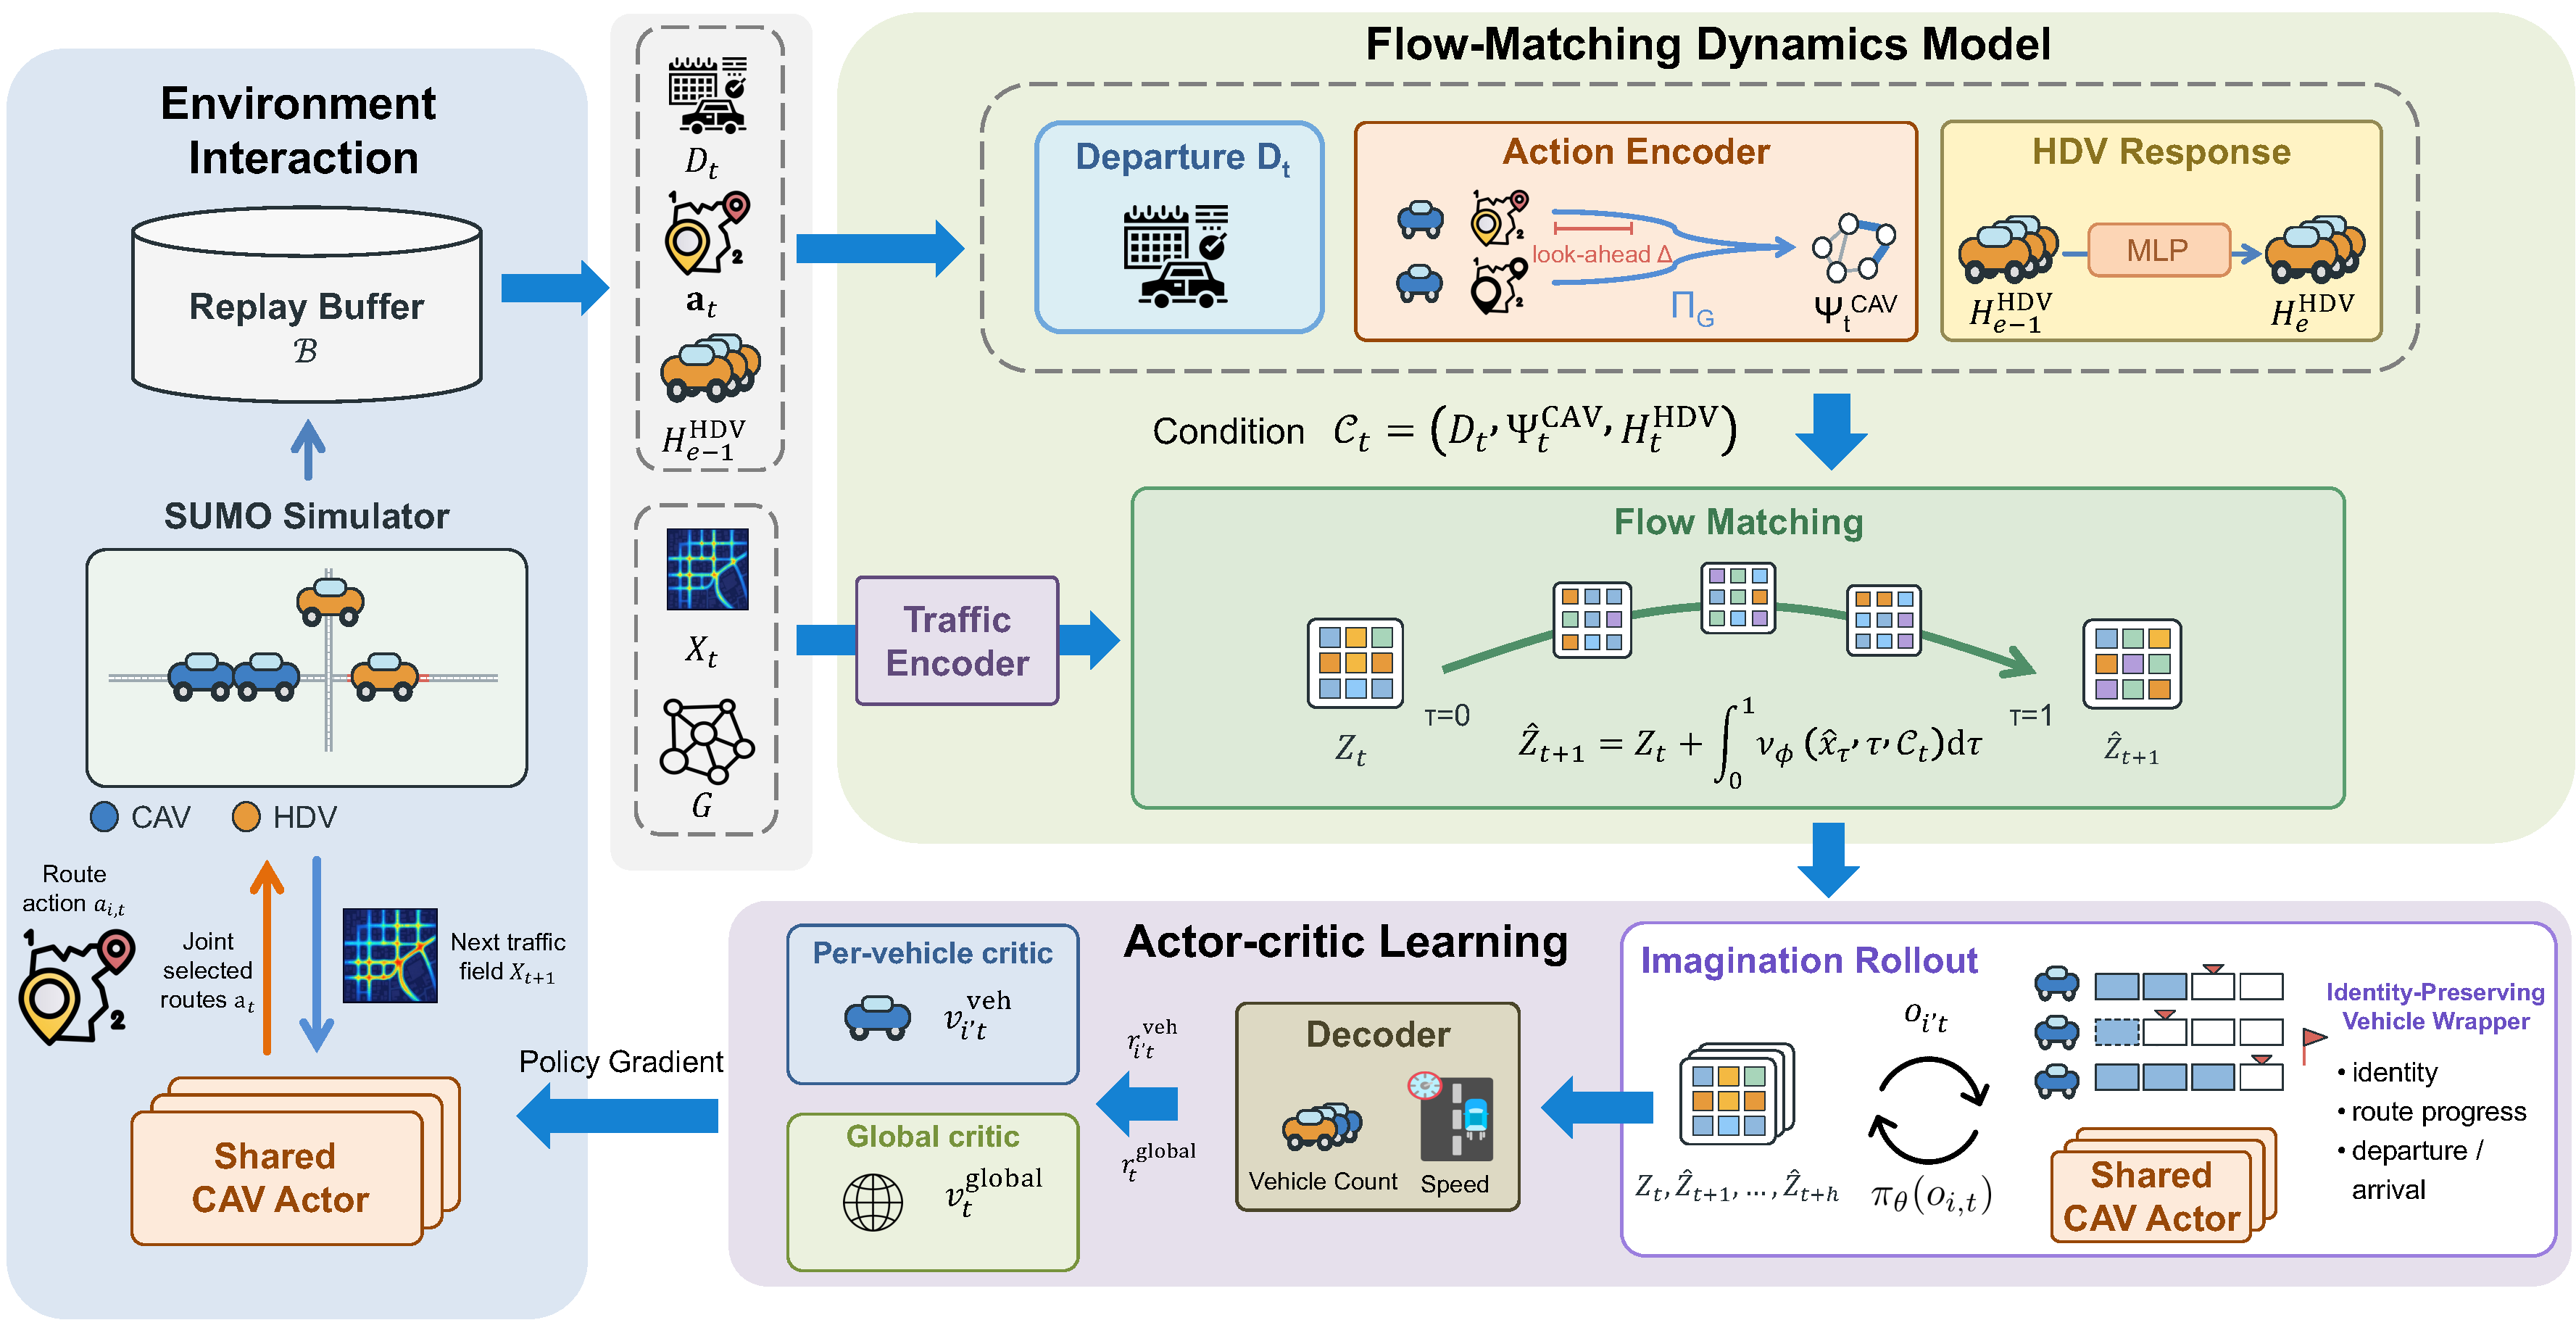
\includegraphics[width=0.8\textwidth]{figure/UrbanDreamer}
  \caption{Overview of UrbanDreamer.}
  \label{fig:architecture}
\end{figure*}


\subsection{Flow Matching Dynamics Model}


\subsubsection{Traffic Encoder and Decoder}

A stack of graph convolution layers with residual connections and layer
normalization maps the traffic field \(X_t\) to the latent representation
\(Z_t\), whose row \(z_{t,u}\) summarizes segment \(u\) together with its
graph neighborhood (Appendix~\ref{app:math-details}).  A decoder maps each
\(z_{t,u}\) back to the dynamic segment attributes
\([\hat c_{t,u},\hat v_{t,u}]\), trained jointly with the dynamics model
through a reconstruction loss on observed traffic fields, and provides the
travel-time and count readouts for rewards and value targets in actor-critic
learning.


\subsubsection{Action Encoder}

The transition model evolves graph-level representations, but decisions are
made at the vehicle level.  We therefore project the realized one-hot CAV
route decisions onto the segment nodes those routes are expected to visit,
producing a planned pressure field \(\Psi_t^{\mathrm{CAV}}\) defined on the
same segment set as \(X_t\) and \(Z_t\).  For active CAV \(i\), let
\(\mathrm{Seg}_{\Delta}(P^k_{i,t})\subseteq N\) denote the segments it would
enter within the look-ahead window \(\Delta\) under candidate \(P^k_{i,t}\);
the planned pressure averages route indicators over the active set:
\begin{equation}
\begin{array}{rcl}
\Psi_t^{\mathrm{CAV}}(u)
=
\displaystyle
\frac{1}{\max(|\mathcal{I}_t|,1)}
\sum_{i\in\mathcal{I}_t}\sum_{k=1}^{K}
\mathbf{1}[k=a_{i,t}]
\displaystyle
\,\xi_{i,t}^{k,\Delta}(u),\\
\xi_{i,t}^{k,\Delta}(u)
=
\left\{
\begin{array}{ll}
1, & u\in\mathrm{Seg}_{\Delta}(P^k_{i,t})\\
0, & \mathrm{otherwise}
\end{array}
\right.
\end{array}
\end{equation}
The same sampled one-hot route is executed by the vehicle, stored in replay,
and supplied to the transition condition, so \(\Psi_t^{\mathrm{CAV}}\)
always matches the physical intervention.  The mean normalization states
where the controlled demand intends to go, not how large it is.



\subsubsection{State-to-State Flow Matching}

UrbanDreamer learns the latent transition with state-to-state flow
matching \cite{GiFlow} under the transition condition
\begin{equation}
\mathcal{C}_t=
(\Psi_t^{\mathrm{CAV}},D_t,H_t^{\mathrm{HDV}}).
\end{equation}
Instead of regressing \(Z_{t+1}\) directly, the model learns a velocity
field that transports the current latent representation to the next one.
For a real transition pair \((Z_t,Z_{t+1})\), sample
\(\tau\sim\mathcal{U}(0,1)\) and define
\begin{equation}
\begin{array}{rcl}
x_\tau &=& (1-\tau)Z_t+\tau Z_{t+1},\\
\nu_{t,\tau} &=& \frac{dx_\tau}{d\tau} = Z_{t+1}-Z_t.
\end{array}
\end{equation}
The previous latent representation \(Z_t\) is the flow source, and
\(\nu_{t,\tau}\) is the target velocity.  This deterministic state-to-state
transport is based on rectified flow \cite{lipman2023flow,liu2023rectified}:
the straight interpolation path keeps multi-step imagined rollouts stable,
and we do not claim multimodal generative modeling of \(Z_{t+1}\).

We parameterize the velocity predictor \(\nu_\phi\) with a block-causal
transformer \cite{vaswani2017attention} over segment traffic
representations, which receives the interpolated representation \(x_\tau\),
the time condition \(\tau\), and the transition condition \(\mathcal{C}_t\),
mixes information through causal attention over previous traffic
representations, and outputs the velocity estimate
\begin{equation}
\hat\nu_{t,\tau}=\nu_\phi(x_\tau,\tau,\mathcal{C}_t).
\end{equation}
Because most road segments are empty most of the time, the training loss
applies bounded per-segment weights \(w_{t,u}\) that emphasize occupied and
congested segments (Appendix~\ref{app:math-details}).

At imagination time, the next latent traffic representation is obtained by
integrating the learned velocity field with \(k\) explicit Euler steps:
\begin{equation}
\begin{array}{rcl}
\hat Z_{t+1}
&=&
\displaystyle
Z_t+\int_0^1
\nu_\phi(\hat x_\tau,\tau,\mathcal{C}_t)\,d\tau.
\end{array}
\end{equation}
Multi-step imagination repeatedly applies this one-step transition, using
each predicted \(\hat Z_{t+1}\) as the next source representation.
% 中文注释：想象阶段从 \(x_0=Z_t\) 对速度场做 ODE 积分；多步想象反复应用一步 transition。


\subsection{HDV Response Module}

HDVs choose routes at departure time and adapt across episodes to the
congestion that CAV routing induces.  UrbanDreamer models the two time
scales separately.  Within an episode, the learned transition responds to
the current CAV pressure \(\Psi_t^{\mathrm{CAV}}\) at every decision epoch.
Across episodes, slower human adaptation is represented as an episode-level
response field over road segments, predicted from the previous episode and
held fixed within each imagined episode.  Imagined rollouts therefore
optimize against step-level counterfactual traffic responses, while
day-to-day HDV demand shifts are learned from real simulator episodes
rather than simulated inside imagination.

The HDV influence is represented as a road-segment distribution
\(H^{\mathrm{HDV}}\): the supervision target \(H^\star\) aggregates the
observed HDV background field over an episode and normalizes it across
segments, and an MLP with a softmax output estimates
\(\hat H_e^{\mathrm{HDV}}\) from the previous episode's CAV pressure summary
and HDV background.  The predictor is trained with a soft-label
cross-entropy loss and an optimizer separate from the world model, so HDV
adaptation is learned without treating HDVs as controllable
(Appendix~\ref{app:math-details}).




\subsection{Actor-Critic Learner}

The learner runs the following loop inside the learned model.  An imagined
rollout is generated by the actor, the world model, and a vehicle wrapper;
each imagined step produces a per-vehicle travel-time reward and a
network-level global reward; two centralized critics estimate the
corresponding returns; and the actor is updated from their combined
advantage.  This dense credit is necessary because the global mean travel
time in Definition~7 is an episode-level objective that is available only
after a simulator episode is completed.  The per-vehicle signal is the
primary actor-learning signal, while the global critic supplies an auxiliary
aggregate value signal.
% 中文注释：学习循环：actor、world model 和 vehicle wrapper 生成 imagined rollout；每个 imagined step 产生 per-vehicle travel-time reward 和 network-level global reward；两个 centralized critics 估计对应 returns;actor 用组合 advantage 更新。需要 dense credit 是因为 Definition~7 的 global mean travel time 是 episode 级目标，只有 simulator episode 完成后才能获得。per-vehicle signal 是主要 actor-learning signal,global critic 提供辅助的 aggregate value signal。

\subsubsection{Vehicle-Level Imagination}

Imagined rollouts start from a replay state: we sample a replay episode and a
decision epoch \(t_{\mathrm{start}}\), encode the aligned traffic field as
\(Z_{t_{\mathrm{start}}}=f_\phi(X_{t_{\mathrm{start}}},G)\), and initialize
each vehicle's current segment, destination, route suffix, and arrival status
from the same epoch.  At each imagined epoch, the actor selects a route and
the decoder recovers the segment speed \(\widehat v_{t,u}\), giving the
predicted segment travel time
\begin{equation}
\begin{array}{rcl}
\widehat\tau_t(u)
&=&
\displaystyle
\frac{\ell(u)}{\widehat v_{t,u}}.
\end{array}
\end{equation}
During a decision interval \(\Delta t\), a deterministic vehicle wrapper
advances each vehicle along its selected route by consuming these travel times
in route order, while the learned transition predicts \(Z_{t+1}\).  Because
the wrapper and the transition consume the same decoded readout, vehicle
positions and the segment traffic field evolve from a single prediction rather
than two independent state estimates.  Vehicles reaching their departure time
are added at the next epoch and arrived vehicles are removed; the remaining
CAVs form \(\mathcal{I}_{t+1}^{\mathrm{im}}\) and alone contribute actor
samples, rewards, and bootstrap values.  This wrapper keeps vehicle identity
explicit without requiring the graph-level world model to predict per-vehicle
terminal variables.
% 中文注释：imagined rollout 从 replay state 初始化：采样 replay episode 和 decision epoch \(t_{\mathrm{start}}\)，编码 \(Z_{t_{\mathrm{start}}}=f_\phi(X_{t_{\mathrm{start}}},G)\)，并从同一 epoch 初始化每辆车的 current segment、destination、route suffix 和 arrival status。每个 imagined epoch,actor 选择 route,decoder 给出 segment speed \(\widehat v_{t,u}\) 和 travel time \(\widehat\tau_t(u)=\ell(u)/\widehat v_{t,u}\)。deterministic vehicle wrapper 在 \(\Delta t\) 内按 route 顺序消耗这些 travel time 推进车辆，同时 transition 预测 \(Z_{t+1}\);wrapper 与 transition 共享同一 decoded readout，因此车辆位置与 segment field 来自同一个预测。到点车辆加入、到达车辆移除，剩余 CAV 构成 \(\mathcal{I}_{t+1}^{\mathrm{im}}\)。该 wrapper 在不要求 world model 预测 per-vehicle terminal variables 的情况下显式保留 vehicle identity。

\subsubsection{Imagined Rewards}

For the route selected by CAV \(i\), let \(P_{i,t}^{\mathrm{rem}}\) denote its
suffix road segments.  The per-vehicle reward charges the imagined travel time
accumulated before the next decision or arrival:
\begin{equation}
\begin{array}{rcl}
\widehat T_{i,t}^{\mathrm{rem}}
&=&
\displaystyle
\sum_{u\in P_{i,t}^{\mathrm{rem}}}
\widehat\tau_{t+1}(u),\\[0.35em]
\delta_{i,t}
&=&
\min(\Delta,\widehat T_{i,t}^{\mathrm{rem}}),\\
r_{i,t}^{\mathrm{veh}}
&=&
-\delta_{i,t}/\kappa_r,
\end{array}
\end{equation}
where \(\kappa_r\) controls the reward scale.
% 中文注释：per-vehicle reward 由 \(\delta_{i,t}=\min(\Delta,\widehat T_{i,t}^{\mathrm{rem}})\) 和 \(r_{i,t}^{\mathrm{veh}}=-\delta_{i,t}/\kappa_r\) 给出，其中 \(\widehat T_{i,t}^{\mathrm{rem}}\) 是所选 route 剩余 suffix 的 predicted travel time。

The global reward charges each decision interval by the travel time
accumulated by all vehicles present in the network:
\begin{equation}
\begin{array}{rcl}
r_t^{\mathrm{global}}
&=&
\displaystyle
-\kappa_g\,
\frac{N_{\mathrm{active}}(t)\,\Delta t}{N_{\mathrm{veh}}},
\end{array}
\end{equation}
where \(N_{\mathrm{veh}}\) is the episode vehicle population and \(\kappa_g\)
controls the reward scale.  On real transitions, \(N_{\mathrm{active}}(t)\) is
read directly from the simulator state.  In imagined rollouts, it is computed
from the decoded count field, \(N_{\mathrm{active}}(t)=\sum_{u\in N}\widehat
n_{t,u}\) with \(\widehat n_{t,u}=\kappa(u)\hat c_{t,u}\).  Since \(\sum_t
N_{\mathrm{active}}(t)\Delta t\) is the total travel time accumulated over an
episode, the sum of \(r_t^{\mathrm{global}}\) equals \(-\kappa_g\) times the
global mean travel time of Definition~7.  Both rewards are therefore computed
from the decoded readouts rather than learned.
% 中文注释：global reward 按当前网络中所有车辆累计的通行时间对每个 decision interval 计费：\(r_t^{\mathrm{global}}=-\kappa_g N_{\mathrm{active}}(t)\Delta t/N_{\mathrm{veh}}\)。真实 transition 上 \(N_{\mathrm{active}}(t)\) 直接从 simulator 读取；imagined rollout 中用 decoded count field 求和 \(\sum_u\widehat n_{t,u}\),\(\widehat n_{t,u}=\kappa(u)\hat c_{t,u}\)。由于 \(\sum_t N_{\mathrm{active}}(t)\Delta t\) 是整个 episode 累计的总通行时间，\(r_t^{\mathrm{global}}\) 的求和等于 \(-\kappa_g\) 倍的 Definition~7 global mean travel time。两种 reward 都由 decoded readouts 计算得到，不需要学习。

\subsubsection{Critics}

The per-vehicle critic first encodes every observation independently with a
parameter-shared multilayer perceptron (MLP) \(f_\eta^{\mathrm{enc}}\), and then
applies multi-head self-attention within the active CAV set:
\begin{equation}
\begin{array}{rcl}
e_{i,t} &=& f_\eta^{\mathrm{enc}}(o_{i,t}),\\
(\widetilde e_{i,t})_{i\in\mathcal{I}_t}
&=&
\mathrm{Attention}_\eta((e_{i,t})_{i\in\mathcal{I}_t}),\\
v_{i,t}^{\mathrm{veh}}
&=&
w_v^\top\widetilde e_{i,t}+b_v.
\end{array}
\end{equation}
The attention layer lets each value estimate account for simultaneous CAV
decisions and route overlap, while \(v_{i,t}^{\mathrm{veh}}\) remains a
per-vehicle estimate of the future return.  It is trained by lambda returns
linked by vehicle identity: only observations of the same CAV are connected by
the recursion, and bootstrapping stops once the vehicle leaves the active set
(Appendix~\ref{app:math-details}).
% 中文注释：per-vehicle critic 先用 parameter-shared MLP 独立编码每个 observation，再在 active CAV set 内做 multi-head self-attention，使每个 value 能考虑 simultaneous decisions 和 route overlap，但仍为每辆车输出一个 value。它用按 vehicle identity 连接的 lambda returns 训练；车辆离开 active set 后停止 bootstrap。

The auxiliary global critic reuses the graph representation \(\bar z_t\):
\begin{equation}
\begin{array}{rcl}
v_t^{\mathrm{global}}
&=&
V_\omega^{\mathrm{global}}
(\bar z_t).
\end{array}
\end{equation}
The planned CAV pressure \(\Psi_t^{\mathrm{CAV}}\) conditions only the
world-model transition and never enters a value baseline, so
\(v_t^{\mathrm{global}}\) is an action-independent estimate of the
network-level state value.  The global critic captures aggregate congestion
effects that cannot be assigned to one CAV observation alone.  It is trained
from the corresponding epoch-level lambda return
(Appendix~\ref{app:math-details}), and its detached residual enters every
active CAV's actor advantage below.
% 中文注释：辅助 global critic 复用 graph representation \(\bar z_t\)：\(v_t^{\mathrm{global}}=V_\omega^{\mathrm{global}}(\bar z_t)\)。planned CAV pressure 只作为 world-model transition 的条件，不进入任何 value baseline，因此 \(v_t^{\mathrm{global}}\) 是 action-independent 的 network-level state value 估计。global critic 用 epoch 级 lambda return 训练，其 detached residual 进入下文每辆 active CAV 的 actor advantage。

\subsubsection{Route Actor and Policy Update}

The actor scores every candidate route from a fixed-dimensional route
representation \(\varphi_{i,t,k}\), obtained by mean pooling the segment
latents along the route, and a shared context \(g_t\) containing the pooled
graph latent, the normalized decision time, and the active-CAV fraction
(Appendix~\ref{app:math-details}).  The learned policy must select one
executable route at deployment, so the scores are normalized into a
categorical distribution over the valid candidates:
\begin{equation}
\begin{array}{rcl}
\pi_\theta(k\mid o_{i,t})
&=&
\mathrm{Softmax}_{k:m_{i,t,k}=1}
\!\left(f_\theta^{\mathrm{route}}(\varphi_{i,t,k},g_t)\right).
\end{array}
\end{equation}
Candidates with \(m_{i,t,k}=0\) are excluded from the softmax, and invalid
slots are masked out when fewer than \(K\) candidates exist.  Parameter
sharing across CAVs and candidate slots keeps the policy applicable to a
variable number of active vehicles.
% 中文注释：actor 从 mean-pooled route representation \(\varphi_{i,t,k}\) 和 shared context \(g_t\) 为每条候选打分，并对有效候选做 masked softmax:\(\pi_\theta(k\mid o_{i,t})=\mathrm{Softmax}_{k:m_{i,t,k}=1}(f_\theta^{\mathrm{route}}(\varphi_{i,t,k},g_t))\)。\(m_{i,t,k}=0\) 的候选不参与 softmax；候选不足 \(K\) 时无效 slot 被 mask。CAV 与候选 slot 之间的 parameter sharing 使 policy 适用于可变数量的 active vehicles。

For policy optimization, let \(\pi_{\mathrm{old}}\) denote the behavior policy
that produced \(a_{i,t}\).  The detached per-vehicle and global advantages and
their actor combination are
\begin{equation}
\begin{array}{rcl}
A_{i,t}^{\mathrm{veh}}
&=&
\mathrm{sg}\!\left(
G_{i,t}^{\lambda}-v_{i,t}^{\mathrm{veh}}
\right),\\
A_t^{\mathrm{global}}
&=&
\mathrm{sg}\!\left(
G_t^{\mathrm{global}}-v_t^{\mathrm{global}}
\right),\\
A_{i,t}^{\mathrm{actor}}
&=&
A_{i,t}^{\mathrm{veh}}+\alpha_g A_t^{\mathrm{global}},
\end{array}
\end{equation}
where \(G_{i,t}^{\lambda}\) and \(G_t^{\mathrm{global}}\) are the lambda-return
targets of the two critics, \(\mathrm{sg}\) stops gradients through the return
targets, and \(\alpha_g\) weights the global credit shared by CAV actions from
the same imagined epoch, so policy improvement internalizes network-wide
congestion while retaining vehicle-specific credit.  The actor is optimized
with the standard clipped PPO surrogate with entropy regularization
(Appendix~\ref{app:math-details}).  Thus the global critic affects the actor
through \(A_t^{\mathrm{global}}\), rather than only through a critic loss.
% 中文注释：vehicle advantage 与 global advantage 分别为 \(A_{i,t}^{\mathrm{veh}}=\mathrm{sg}(G_{i,t}^{\lambda}-v_{i,t}^{\mathrm{veh}})\) 和 \(A_t^{\mathrm{global}}=\mathrm{sg}(G_t^{\mathrm{global}}-v_t^{\mathrm{global}})\),actor 使用 \(A_{i,t}^{\mathrm{actor}}=A_{i,t}^{\mathrm{veh}}+\alpha_gA_t^{\mathrm{global}}\)。\(\mathrm{sg}\) 阻断 return targets 上的梯度，\(\alpha_g\) 控制 global credit 的权重；同一 imagined epoch 的 active CAVs 共享 global term，因此 policy update 同时保留 vehicle-specific credit 并纳入 network-wide congestion credit。actor 用标准 clipped PPO surrogate 加 entropy regularization 优化(附录)。global critic 不只产生 critic loss，它的 detached lambda advantage 直接进入 actor objective。



\section{Experiments}

We evaluate UrbanDreamer in the SUMO traffic simulator \cite{lopez2018microscopic} on three urban road networks, covering sample and computational efficiency, final routing quality, and ablations.

\subsection{Experimental Settings}

\subsubsection{Datasets and Road Networks}

We use three urban road networks from the RouteRL and URB benchmarks \cite{akman2025routerl,akman2026urb}: Gretz-Armainvilliers (4,485 road segments, 636 agents), Ingolstadt \cite{lobo2020intas} (853 segments, 1,035 agents), and Fontenay-en-Parisis (7,585 segments, 2,068 agents), with CAV penetration fixed at 40\%. To create congested bottlenecks, temporary speed reductions are imposed on selected SUMO edges following a fixed within-episode schedule, identical across episodes and shared by all methods, so they act as a stationary property of each benchmark rather than an exogenous stochastic event.


\subsubsection{Baselines}

We compare against two heuristics and four MARL methods. Free-flow greedy selects the candidate route with the minimum sum of free-flow travel times, and live-current greedy uses current travel-time estimates. The learning baselines are IQL \cite{iql}, IPPO \cite{ippo}, MAPPO \cite{mappo}, and MAMBA \cite{mamba}, covering independent value learning, decentralized policy optimization, and centralized training with decentralized execution; MAMBA is a Dreamer-style multi-agent model-based method and serves as the direct world-model baseline. All methods share the same route-candidate interface, departure demand, and disruption schedule, are trained under the same protocol until convergence, and are evaluated on identical episodes (Appendix~\ref{app:baselines}); the environment-step counts reported below measure each method's online training interactions.

\subsubsection{Evaluation Metrics}

All methods are evaluated with the same route candidates, demand, disruption settings, simulation horizon, and initial HDV state, and the horizon is long enough for every vehicle to arrive. We use the global mean travel time \(T_{\mathrm{all}}\) as the primary metric and additionally report the CAV mean travel time \(T_{\mathrm{CAV}}\), the added cost \(C_{\mathrm{ALL}}\) relative to the pre-CAV reference state, measured on training episodes and therefore defined only for the learning-based methods, and the 95th-percentile travel time \(T_{\mathrm{P95}}\).  A negative \(C_{\mathrm{ALL}}\) indicates that the learned routing reduces the cost below the pre-CAV reference. Multi-seed stability and hyperparameter sensitivity analyses are reported in Appendix~\ref{app:additional-experiments}.


\subsection{Efficiency and Scalability}

\subsubsection{Sample Efficiency}

We measure sample efficiency by the number of real SUMO environment steps each method requires to converge, where convergence is the episode at which the 20-episode moving-average \(T_{\mathrm{all}}\) first reaches its best value during training, and the same criterion is applied identically to every method.

\begin{table}[t]
  \centering
  \caption{Sample efficiency on the three urban networks. Lower values indicate better performance; the best value in each column is in bold.}
  \renewcommand{\arraystretch}{1.0}
  \renewcommand{\arraystretch}{1.0}
  \setlength{\tabcolsep}{12pt}
    \begin{tabular}{lccc}
    \toprule
    \multirow{2}{*}{Method} & \multicolumn{3}{c}{Environment Steps $\downarrow$} \\
    & Gretz & Ingolstadt & Fontenay \\
      \midrule
      IQL & 13,320 & 11,040 & 4,680 \\
      IPPO & 9,240 & 10,560 & 11,040 \\
      MAPPO & 3,540 & 3,300 & 3,720 \\
      MAMBA & 8,760 & 12,600 & 6,660 \\
      \textbf{UrbanDreamer} & \textbf{2,040} & \textbf{2,220} & \textbf{2,160} \\
      \bottomrule
    \end{tabular}
  \label{tab:sample-efficiency}
\end{table}


Figure~\ref{fig:sample-efficiency-training-proxy} shows the training curves, and Table~\ref{tab:sample-efficiency} reports the environment steps required to reach convergence. UrbanDreamer requires 5,400, 5,700, and 7,320 steps on Gretz-Armainvilliers, Ingolstadt, and Fontenay-en-Parisis, respectively, reducing the required steps by 77.2\%, 77.3\%, and 69.8\% relative to the baseline with the fewest steps on each network.

\begin{figure*}[t]
  \centering
  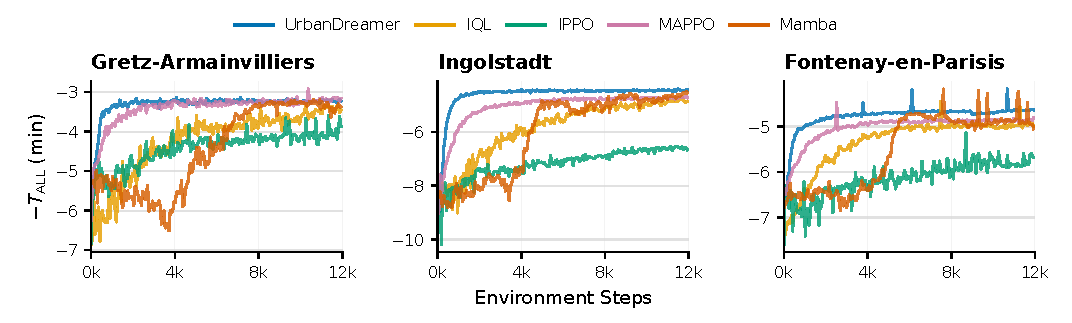
\includegraphics[width=0.8\textwidth]{figure/sample_efficiency.pdf}
  \caption{Training curves over real SUMO environment steps on the three urban networks. UrbanDreamer reaches its best moving-average $T_{\mathrm{all}}$ with 69.8\%--77.3\% fewer steps than the most sample-efficient baseline on each network.}
  \label{fig:sample-efficiency-training-proxy}
\end{figure*}



\subsubsection{Computational Efficiency}

\begin{table}[t]
  \centering
  \caption{Computational efficiency on the three urban networks. All runs use a single NVIDIA RTX 3090 GPU. Lower is better; best in bold.}
  \renewcommand{\arraystretch}{1.0}
  \setlength{\tabcolsep}{12pt}
  \begin{tabular}{lccc}
    \toprule
    \multirow{2}{*}{Method} & \multicolumn{3}{c}{Total Training Time (hours) $\downarrow$} \\
    & Gretz & Ingolstadt & Fontenay \\
    \midrule
    IQL & 28.8 & 15.3 & 78.2 \\
    IPPO & 33.0 & 10.4 & 96.1 \\
    MAPPO & 35.1 & 13.9 & 85.6 \\
    MAMBA & 37.0 & 10.2 & 78.9 \\
    \textbf{UrbanDreamer} & \textbf{17.4} & \textbf{5.6} & \textbf{33.3} \\
    \bottomrule
  \end{tabular}
  \label{tab:computation-efficiency}
\end{table}

Table~\ref{tab:computation-efficiency} reports the training time to convergence of each learning method (per-stage breakdown in Appendix~\ref{app:architecture}). UrbanDreamer completes training in 19.0, 5.4, and 36.6 hours on the three networks, reducing training time by 36.0\%, 48.1\%, and 49.2\% relative to the fastest baseline on each network.


\subsubsection{Scalability with Traffic-System Size}

\begin{figure}[t]
  \centering
  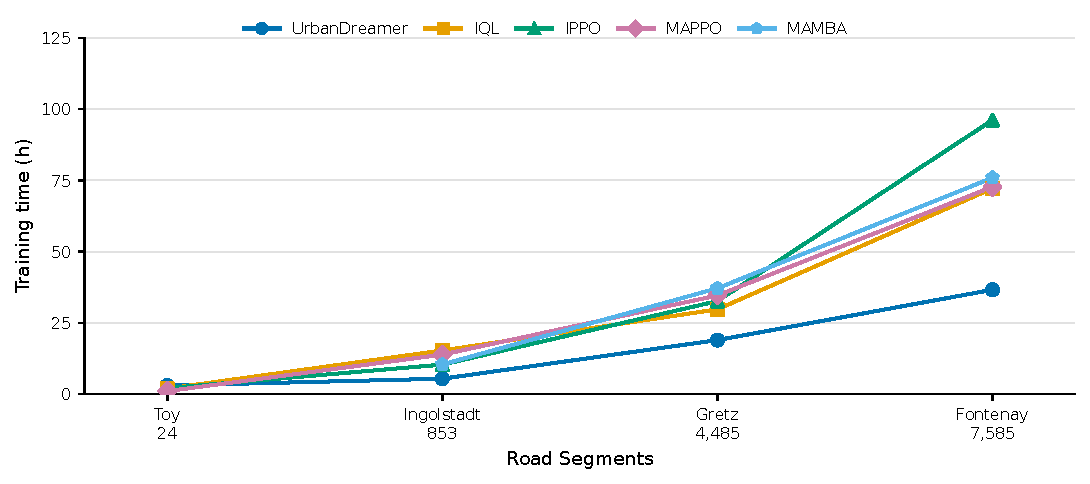
\includegraphics[width=1.0\linewidth]{figure/scalability_training_time}
  \caption{Total training time across networks of increasing size. The horizontal axis contains four discrete benchmarks ordered by road-segment count: Toy (24), Ingolstadt (853), Gretz-Armainvilliers (4,485), and Fontenay-en-Parisis (7,585). Toy is a small synthetic network used only as a pilot point in this profile. Connecting segments are visual guides rather than interpolation over a continuous scale.}
  \label{fig:scalability_training_time}
\end{figure}

Figure~\ref{fig:scalability_training_time} compares training time across networks of increasing size. Training time grows for all methods, but UrbanDreamer remains consistently faster, and its advantage widens with network size: from 5.4 hours on Ingolstadt to 36.6 hours on Fontenay-en-Parisis (7,585 segments), whereas the baselines require 72.1--96.2 hours on the largest network.

\subsection{Final Routing Quality}

\begin{table*}[t]
  \centering
  \caption{Final routing quality on the three urban networks: mean travel times in minutes for all vehicles, CAVs, and HDVs, and the 95th-percentile travel time \(T_{\mathrm{P95}}\). Lower values indicate better performance; the best value in each column is in bold.}
  \renewcommand{\arraystretch}{1.0}
  \resizebox{1.0\linewidth}{!}{
    \begin{tabular}{lcccccccccccc}
      \toprule
      \multirow{2}{*}{Method} & \multicolumn{4}{c}{Gretz-Armainvilliers} & \multicolumn{4}{c}{Ingolstadt} & \multicolumn{4}{c}{Fontenay-en-Parisis} \\
      \cmidrule(lr){2-5} \cmidrule(lr){6-9} \cmidrule(lr){10-13}
      & $T_{\mathrm{all}}\!\downarrow$ & $T_{\mathrm{CAV}}\!\downarrow$ & $T_{\mathrm{HDV}}\!\downarrow$ & $T_{\mathrm{P95}}\!\downarrow$ & $T_{\mathrm{all}}\!\downarrow$ & $T_{\mathrm{CAV}}\!\downarrow$ & $T_{\mathrm{HDV}}\!\downarrow$ & $T_{\mathrm{P95}}\!\downarrow$ & $T_{\mathrm{all}}\!\downarrow$ & $T_{\mathrm{CAV}}\!\downarrow$ & $T_{\mathrm{HDV}}\!\downarrow$ & $T_{\mathrm{P95}}\!\downarrow$\\
      \midrule
      Free-flow greedy & 3.262 & 3.537 & 3.079 & 6.667 & 4.542 & 4.590 & 4.509 & 7.333 & 4.682 & 4.676 & 4.687 & 22.651\\
      Live-current greedy & 3.331 & 3.710 & 3.079 & 6.950 & \textbf{4.410} & 4.375 & \textbf{4.433} & \textbf{6.616} & 4.691 & 4.693 & 4.690 & 22.636\\
      IQL & 3.321 & 3.687 & 3.078 & 6.867 & 4.595 & 4.785 & 4.468 & 7.416 & 4.968 & 5.552 & 4.577 & \textbf{20.947}\\
      IPPO & 3.933 & 5.169 & 3.111 & 10.569 & 5.679 & 7.532 & 4.443 & 14.693 & 5.438 & 6.611 & 4.657 & 25.171\\
      MAPPO & 3.246 & 3.538 & \textbf{3.050} & 6.617 & 4.664 & 4.867 & 4.528 & 7.533 & 4.838 & 5.245 & 4.566 & 22.928\\
      MAMBA & 3.353 & 3.725 & 3.106 & 6.867 & 4.555 & 4.519 & 4.578 & 7.016 & 5.068 & 5.821 & 4.566 & 23.233\\
      \textbf{UrbanDreamer} & \textbf{3.167} & \textbf{3.297} & 3.081 & \textbf{6.583} & 4.421 & \textbf{4.370} & 4.454 & 6.883 & \textbf{4.600} & \textbf{4.665} & \textbf{4.556} & 22.285\\
      \bottomrule
    \end{tabular}
  }
  \label{tab:overall-performance}
\end{table*}


Table~\ref{tab:overall-performance} reports final routing quality on the three networks. UrbanDreamer attains the lowest global mean travel time on Gretz-Armainvilliers and Fontenay-en-Parisis; on Ingolstadt it is second to live-current greedy by 0.01 minutes and lowest among the learning-based methods. The gains come primarily from lower CAV travel times, and UrbanDreamer also incurs the lowest added cost \(C_{\mathrm{ALL}}\) on all three networks.


\subsection{Ablation}

We conduct three groups of ablations: component ablation on final routing quality, efficiency ablation isolating world-model imagination, and transition ablation comparing predictive quality across transition models.

\subsubsection{Component Ablation}

We compare UrbanDreamer with four variants: Actor-Critic removes world-model imagination, w/o HDV Response removes HDV influence prediction, Vehicle Critic Only retains only the per-vehicle critic, and MSE Transition replaces flow matching with deterministic next-state regression.

\begin{table*}[t]
  \centering
  \caption{Component ablation: final mean travel times in minutes when individual components are removed or replaced. Lower values indicate better performance.}
  \renewcommand{\arraystretch}{1.0}
  \resizebox{1.0\linewidth}{!}{
    \begin{tabular}{lccccccccc}
      \toprule
      \multirow{2}{*}{Method} & \multicolumn{4}{c}{Gretz-Armainvilliers} & \multicolumn{4}{c}{Ingolstadt} & \multicolumn{4}{c}{Fontenay-en-Parisis} \\
      \cmidrule(lr){2-5} \cmidrule(lr){6-9} \cmidrule(lr){10-13}
      & $T_{\mathrm{ALL}}\!\downarrow$ & $T_{\mathrm{CAV}}\!\downarrow$ & $C_{\mathrm{ALL}}\!\downarrow$ & $T_{\mathrm{P95}}\!\downarrow$ & $T_{\mathrm{ALL}}\!\downarrow$ & $T_{\mathrm{CAV}}\!\downarrow$ & $C_{\mathrm{ALL}}\!\downarrow$ & $T_{\mathrm{P95}}\!\downarrow$ & $T_{\mathrm{ALL}}\!\downarrow$ & $T_{\mathrm{CAV}}\!\downarrow$ & $C_{\mathrm{ALL}}\!\downarrow$ & $T_{\mathrm{P95}}\!\downarrow$\\
      \midrule
      Actor-Critic & 3.219 & 3.514 & 0.942 & 6.852 & 4.572 & 4.764 & 4.443 & 4.771 & 5.114 & 4.543 \\
      w/o HDV Response & 3.284 & 3.624 & 0.364 & 6.450 & 4.507 & 4.522 & 4.497 & 4.704 & 4.919 & 4.561 \\
      Vehicle Critic Only & 3.272 & 3.580 & 0.342 & 6.467 & 4.451 & 4.378 & 4.497 & 4.673 & 4.864 & 4.546 \\
      MSE Transition & 3.240 & 3.479 & 3.081 & 0.375 & 6.550 & 4.518 & 4.514 & 4.682 & 4.862 & 4.563 \\
      \textbf{UrbanDreamer} & \textbf{3.167} & \textbf{3.297} & \textbf{0.230} & \textbf{6.583} & 4.421 & \textbf{4.370} & \textbf{0.146} & 6.883 & \textbf{4.600} & \textbf{4.665} & \textbf{-0.295} & 22.285\\
      \bottomrule
    \end{tabular}
  }
  \label{tab:ablation performance}
\end{table*}


Table~\ref{tab:ablation performance} shows that removing any component degrades routing performance on all three networks. Removing world-model imagination causes the largest degradation on Ingolstadt and Fontenay-en-Parisis, while removing the HDV response module is most harmful on Gretz-Armainvilliers. Replacing flow matching with MSE regression also degrades both routing performance and prediction quality (Table~\ref{tab:wm-prediction-ablation}).

\subsubsection{Efficiency Ablation}

\begin{figure*}[t]
  \centering
  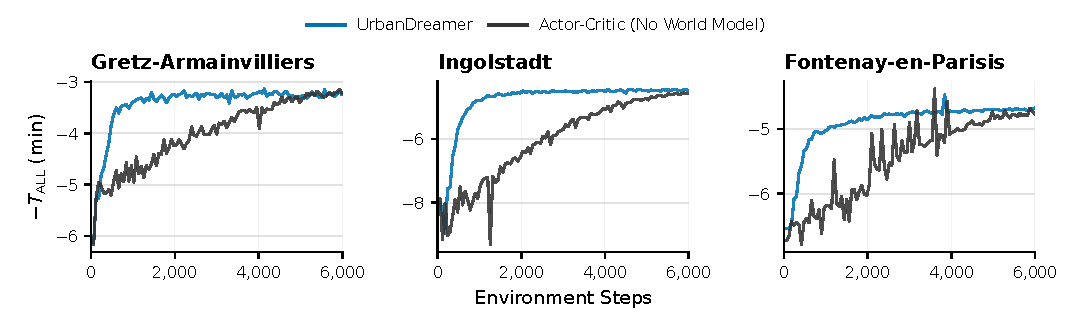
\includegraphics[width=0.8\linewidth]{figure/efficiency_ablation}
  \caption{Sample-efficiency ablation on three urban road networks. The training curves compare UrbanDreamer with Actor-Critic (No World Model) over real SUMO environment steps. Higher \(-T_{\mathrm{all}}\) indicates better routing performance.}
  \label{fig:efficiency_ablation}
\end{figure*}

Figure~\ref{fig:efficiency_ablation} compares UrbanDreamer with Actor-Critic (No World Model) over real environment steps. UrbanDreamer improves substantially faster and stabilizes with fewer steps on all three networks, demonstrating that world-model imagination drives the sample-efficiency gain.

\subsubsection{Transition Ablation}

We compare the flow-matching transition with its MSE-based counterpart on held-out 8-step rollouts, measuring the MAE of normalized speed and capacity-normalized vehicle count.

\begin{table}[t]
  \centering
  \caption{8-step frozen-trace prediction error (lower is better).}
  \renewcommand{\arraystretch}{1.0}
  \resizebox{\columnwidth}{!}{%
    \begin{tabular}{lcccc}
      \toprule
      \multirow{2}{*}{Network} & \multicolumn{2}{c}{Speed MAE $\downarrow$} & \multicolumn{2}{c}{Vehicle Count MAE $\downarrow$} \\
      \cmidrule(lr){2-3} \cmidrule(lr){4-5}
      & Flow Matching & MSE Loss & Flow Matching & MSE Loss \\
      \midrule
      Ingolstadt & \textbf{0.408} & 0.433 & \textbf{0.060} & 0.066 \\
      Gretz-Armainvilliers & \textbf{0.274} & 0.473 & \textbf{0.104} & 0.125 \\
      Fontenay-en-Parisis & \textbf{0.209} & 0.233 & \textbf{0.107} & 0.112 \\
      \bottomrule
    \end{tabular}%
  }
  \label{tab:wm-prediction-ablation}
\end{table}

Table~\ref{tab:wm-prediction-ablation} shows that flow matching achieves lower speed and vehicle-count MAE on all three networks, demonstrating more accurate multi-step transition prediction.

\section{Conclusion}

We presented UrbanDreamer, a world-model-based MARL framework for mixed-autonomy dynamic routing. UrbanDreamer connects vehicle-level route choices with graph-level traffic dynamics through planned CAV pressure, models aggregate HDV responses, and optimizes CAV policies through imagined rollouts with complementary vehicle-level and global critics. Experiments in three SUMO urban networks show that UrbanDreamer learns effective routing policies with substantially fewer real environment steps and less training time than MARL baselines, and attains the lowest global mean travel time on two of the three networks. The ablation results further demonstrate the contributions of world-model imagination and the main model components, while the transition analysis shows that flow matching improves multi-step traffic prediction over deterministic regression. Future work will investigate uncertainty-aware imagination, adaptation across traffic demands and road networks, and deployment under real-world traffic observations.

\section{Limitations}
Our evaluation is conducted in microscopic simulation, and policies are
trained and evaluated separately on each network, so transfer across networks
and demand shifts remains open.




\bibliographystyle{ACM-Reference-Format}
\bibliography{references}


%%
%% If your work has an appendix, this is the place to put it.
\appendix

\section{Training Pipeline}

UrbanDreamer follows a two-stage training pipeline.  The first stage provides warmup learning for the dynamics model. The second stage
alternates real simulator collection, causal HDV-response learning, online
world-model updates, and imagined actor-critic optimization after every
collected episode. Consequently, the model is continually adapted to the
state-action distribution induced by the improving CAV policy, while policy
learning remains grounded in newly observed traffic transitions.
% 中文注释：UrbanDreamer 采用两阶段训练流程。第一阶段为 traffic world model 提供稳定的初始化。第二阶段在每个 collected episode 之后，依次交替进行 real simulator collection、causal HDV-response learning、online world-model updates 和 imagined actor-critic optimization。因此，world model 会持续适应不断改进的 CAV policy 所诱导的 state-action distribution，而 policy learning 仍以新观测到的 traffic transitions 为基础。

\subsubsection{Offline Warmup}

Before online policy learning, we collect a fixed set of transitions from the simulator using exploratory CAV route choices. The encoder, flow-matching dynamics, and decoder are
then fitted on these transitions using \(\mathcal{L}_\phi\). 
% 中文注释：在 online policy learning 之前，我们从 post-mutation simulator state 收集一组固定 transitions；该阶段使用 exploratory CAV route choices，并冻结 HDV adaptation。随后，encoder、flow-matching dynamics 和 decoder 使用 \(\mathcal{L}_\phi\) 在这些 transitions 上完成初始化训练。causal HDV response predictor 不在该阶段训练，因为固定 collection 不能表示由持续变化的 CAV policy 引起的 episode-to-episode response。actor、critics 和 response predictor 在逐 episode online stage 开始时初始化。

\subsubsection{Online Training}

During online collection, HDV adaptation is enabled and the current actor
stochastically samples a valid route for every active CAV.  The same sampled
one-hot decision is used to reroute the vehicle, construct
\(\Psi_{e,t}^{\mathrm{CAV}}\), and store the world-model action in replay.
This action alignment ensures that each observed transition is paired with the
physical CAV intervention that actually produced it.  Deterministic masked
argmax is reserved for simulator evaluation rather than training collection.
% 中文注释：在 online collection 中，HDV adaptation 被启用，current actor 为每辆 active CAV 随机采样一条有效 route。同一个 sampled one-hot decision 同时用于对车辆执行 rerouting、构造 \(\Psi_{e,t}^{\mathrm{CAV}}\)，以及在 replay 中保存 world-model action。这样的 action alignment 保证每个 observed transition 都与实际产生它的物理 CAV intervention 配对。deterministic masked argmax 仅用于 simulator evaluation，而不用于 training collection。

Only episodes satisfying the replay acceptance criterion are admitted to the
bounded world-model replay buffer \(\mathcal{B}\).  Before the observed target
\(H_e^\star\) of an accepted episode is exposed to the response predictor,
\(\hat H_e^{\mathrm{HDV}}\) is computed using only summaries from preceding
episodes and is attached to that episode's transitions.  After
\(H_e^\star\) is recorded, the predictor is updated on the available adjacent
episode pairs using \(\mathcal{L}_\psi\), and the world model is independently
updated on real transition minibatches from \(\mathcal{B}\) using
\(\mathcal{L}_\phi\).  This ordering prevents the current HDV target from
leaking into its own causal prediction.
% 中文注释：只有满足 replay acceptance criterion 的 episodes 才会进入有界的 world-model replay buffer \(\mathcal{B}\)。在 accepted episode 的 observed target \(H_e^\star\) 暴露给 response predictor 之前，\(\hat H_e^{\mathrm{HDV}}\) 只根据先前 episodes 的 summaries 计算，并附加到当前 episode 的 transitions 上。记录 \(H_e^\star\) 后，predictor 使用 \(\mathcal{L}_\psi\) 在已有的 adjacent episode pairs 上更新；world model 则使用 \(\mathcal{L}_\phi\) 在从 \(\mathcal{B}\) 采样的 real transition minibatches 上独立更新。这个顺序防止 current HDV target 泄漏到它自身的 causal prediction 中。

The main online configuration does not apply a direct actor update to real
simulator returns.  Instead, valid CAV decision states are sampled from
\(\mathcal{B}\) to initialize the vehicle-level imagined rollouts described
above.  Within each rollout, the actor samples masked route actions, the same
one-hot actions define the vehicle wrapper and graph-level CAV pressure, and
the world model predicts the resulting traffic evolution.  The resulting
per-vehicle and global lambda returns jointly update the actor and both
critics.
% 中文注释：当前 online 主线不直接使用 real simulator returns 更新 actor。相反，训练从 \(\mathcal{B}\) 中采样包含有效 CAV decisions 的 states，并用它们初始化前文介绍的 vehicle-level imagined rollouts。在每个 rollout 内，actor 采样 masked route actions；相同的 one-hot actions 同时用于 vehicle wrapper 和 graph-level CAV pressure；world model 则预测由这些 actions 导致的 traffic evolution。最终得到的 per-vehicle 和 global lambda returns 共同用于更新 actor 和两个 critics。

\begin{algorithm}[t]
\caption{Online training}
\label{alg:urbandreamer}
\small
\begin{algorithmic}
\REQUIRE Road graph \(G\), simulator, training-episode budget, checkpoint indices
\ENSURE Simulator-selected CAV route actor \(\pi_\theta\)
\FOR{each online episode \(e\)}
  \STATE Collect one simulator episode using masked stochastic route samples from \(\pi_\theta\)
  \STATE Reuse each sampled one-hot route for execution, \(\Psi_{e,t}^{\mathrm{CAV}}\), and replay
  \IF{the episode satisfies the replay acceptance criterion}
    \STATE Predict \(\hat H_e^{\mathrm{HDV}}\) from preceding episode summaries
    \STATE Attach \(\hat H_e^{\mathrm{HDV}}\), append the episode to \(\mathcal{B}\), and discard stale transitions
    \STATE Update \(g_\psi^{\mathrm{HDV}}\) on available adjacent episode pairs
  \ENDIF
  \IF{a world-model update is scheduled and \(\mathcal{B}\) is nonempty}
    \FOR{each configured world-model update}
      \STATE Sample real transitions from \(\mathcal{B}\) and minimize \(\mathcal{L}_\phi\)
    \ENDFOR
  \ENDIF
  \IF{\(\mathcal{B}\) contains enough valid CAV decision states}
    \FOR{each configured imagined actor-critic update}
      \STATE Sample replay start states and initialize their vehicle states
      \FOR{each of the next \(L_{\mathrm{im}}\) imagined decisions}
        \STATE Sample masked routes from \(\pi_\theta\) and construct \(\Psi_t^{\mathrm{CAV}}\)
        \STATE Predict \(Z_{t+1}\) using the stored causal HDV context
        \STATE Advance the vehicle wrapper and record rewards and active masks
      \ENDFOR
      \STATE Compute lambda returns and update the actor and both critics
    \ENDFOR
  \ENDIF
  \IF{\(e\) is a checkpoint episode}
    \STATE Save the actor, critics, world model, and response predictor
  \ENDIF
\ENDFOR
\STATE Evaluate saved actors in the simulator using masked argmax routes
\RETURN The actor with the lowest global mean travel time
\end{algorithmic}
\end{algorithm}
% 中文注释：Algorithm~\ref{alg:urbandreamer} 首先在冻结 HDV adaptation 的固定 warm-up transitions 上初始化 world model。进入 online stage 后，每个 episode 都使用 current actor 的 masked stochastic route samples 进行 simulator collection，并将同一个 sampled one-hot route 用于车辆执行、planned CAV pressure 和 replay。满足 acceptance criterion 的 episode 会先得到仅依赖先前 episode summaries 的 causal HDV prediction，再进入 bounded replay；随后分别更新 HDV response predictor 和 world model。当 replay 中存在足够的有效 CAV decision states 时，算法从 replay 初始化 imagined rollouts，在每一步采样 route、推进 world model 和 vehicle wrapper，并根据 lambda returns 联合更新 actor 与两个 critics。训练完成后，所有 saved actors 使用 masked argmax 在 simulator 中评估，并按照 global mean travel time 选择最终 actor。

At designated episodes, UrbanDreamer saves the actor, critics, world model,
and response predictor together.  After online training, each saved actor is
evaluated in the real simulator with masked argmax route selection, and the
checkpoint with the lowest global mean travel time is selected.  Simulator
selection prevents favorable world-model errors from determining the final
policy solely through imagined returns.
% 中文注释：在指定 episodes，UrbanDreamer 会同时保存 actor、critics、world model 和 response predictor。online training 完成后，每个 saved actor 都使用 masked argmax route selection 在真实 simulator 中评估，并选择 global mean travel time 最低的 checkpoint。基于 simulator 的选择可以防止有利于 policy 的 world-model errors 仅通过 imagined returns 决定最终 policy。


\section{Experimental Settings}
\label{app:exp-settings}

\paragraph{Benchmarks.}  Table~\ref{tab:benchmarks} summarizes the three urban
networks.  All methods use the same departure demand, candidate route
generator (\(K=4\) candidates per decision), and incident configuration.  The
incident speed caps are applied to all lanes of the selected edges during the
indicated window and are removed afterwards; the decision interval is 60~s
for all networks.

\begin{table}[h]
  \centering
  \caption{Benchmark statistics.}
  \renewcommand{\arraystretch}{1.0}
  \resizebox{\columnwidth}{!}{
    \begin{tabular}{lccc}
      \toprule
      & Gretz-Armainvilliers & Ingolstadt & Fontenay-en-Parisis \\
      \midrule
      Road segments & 4,485 & 853 & 7,585 \\
      Scheduled vehicles & 636 & 1,035 & 2,068 \\
      CAVs / HDVs & 254 / 382 & 414 / 621 & 827 / 1,241 \\
      Incident edges & 1 & 1 & 7 \\
      Incident window (s) & [500, 2500) & [500, 1500) & [300, 1800) \\
      Speed cap (m/s) & 0.1 & 1.0 & 0.1 \\
      \bottomrule
    \end{tabular}
  }
  \label{tab:benchmarks}
\end{table}

\paragraph{Training and evaluation protocol.}  The world-model warm-up
collects 50 exploratory episodes in which every CAV follows an
\(\epsilon\)-greedy routing rule (\(\epsilon=0.4\)).  All methods are trained
for 500 episodes per network under the same protocol, saving checkpoints
every 25 episodes.  Each checkpoint is then evaluated with
the same masked stochastic route sampling used in collection, running enough
held-out episodes for the HDV day-to-day route-choice probabilities to
stabilize, and the reported results correspond to the final checkpoint after
convergence.  All runs use a single NVIDIA RTX 3090 GPU.

\paragraph{Toy network.}  The scalability profile additionally includes a
small synthetic Toy network with 24 registered road segments and the same
decision interval and CAV penetration as the real networks.  It serves only
as the smallest pilot point in
Figure~\ref{fig:scalability_training_time} and is not used in any other
experiment.

\section{Baseline Implementations}
\label{app:baselines}

All learning baselines use the same route-candidate observations and valid
candidate masks as UrbanDreamer, and are trained on the same episodes under
the protocol of Appendix~\ref{app:exp-settings}.

\paragraph{Greedy heuristics.}  Free-flow greedy and live-current greedy are
training-free: at each decision they select the valid candidate with the
smallest sum of free-flow or current segment travel times, respectively.

\paragraph{IQL.}  Independent Q-learning with a parameter-shared Q-network
over the route observations.  Exploration is \(\epsilon\)-greedy over valid
candidates, with \(\epsilon\) decayed from \(0.99\) to \(0.05\) per decision.

\paragraph{IPPO.}  Independent PPO with a parameter-shared actor--critic,
probability-ratio clip \(0.2\), and entropy regularization; each CAV learns
from its own transitions.

\paragraph{MAPPO.}  The same decentralized actor as IPPO, trained with a
centralized critic that reads the joint traffic state and outputs a value for
each vehicle slot (three hidden layers of width 64).

\paragraph{MAMBA.}  A Dreamer-style multi-agent model-based baseline using
the upstream architecture defaults: a per-agent discrete latent state model
(\(32\times32\) categoricals) with transformer dynamics (3 layers, 8 heads),
imagination horizon 15, and PPO clip \(0.075\).  Its world model is first
warmed up on 41 exploratory episodes before online training.  Unlike
UrbanDreamer, MAMBA's
learned model is agent-centric: it does not model the segment-level traffic
field or the HDV demand, and its world model, actor, and critic are trained
from the same online episodes as the other baselines.

\section{HDV Adaptation in the Simulator}
\label{app:hdv-adaptation}

Each HDV belongs to one origin--destination (OD) pair with \(K=4\) candidate
routes generated by the same route generator used for CAVs.  At its departure
time, an HDV samples one route from the current per-OD route-choice
probabilities and keeps it for the rest of the episode.  After each episode,
the probabilities of every OD pair are updated once in the day-to-day Gawron
style: each OD pair maintains a route-cost memory \(c\in\mathbb{R}^{K}\),
route probabilities are \(p\propto\exp(\beta c)\) with \(\beta=-1.5\), and the
cost memory moves toward the realized route travel times of the finished
episode, \(c\leftarrow c+\alpha_{0}\,p\odot(\bar t-c)\) with \(\alpha_{0}=0.2\),
where \(\bar t\) is the per-route mean travel time observed in that episode.
Routes not used by any vehicle in an episode are assigned \(1.5\times\) the
worst observed route time.  The information set of the update is therefore
limited to realized travel times, the update frequency is once per episode,
and the same learning state persists across episodes.  During training
evaluation, the adaptation state is checkpointed, frozen, and reloaded
identically before evaluating every compared method.

\section{Architecture Details}
\label{app:architecture}

\paragraph{Encoder and decoder.}  The encoder projects the segment
features to \(d_z=64\) and applies two graph convolution layers over the
row-normalized adjacency matrix (each row sums to one), with messages passed
along the directed edges of the segment-node graph.  The decoder shares a
linear--SiLU block and splits into per-channel heads for the four dynamic
channels; the vehicle-count head applies a softplus map, and the travel-time
readout \(\widehat\tau_t(u)=\ell(u)/\widehat v_{t,u}\) clips the decoded speed
ratio to \([0.05,1.50]\) of the free-flow speed before inversion.

\paragraph{Velocity predictor.}  The velocity predictor is a block-causal
transformer with hidden size 256, 6 layers, and 4 attention heads: segment
latents are packed into spatial tokens, attention mixes tokens within one
decision epoch, and temporal context is attended causally over a sliding
history window of up to \(k_{\max}=8\) past traffic representations.  The
conditions \((\Psi_t^{\mathrm{CAV}},D_t,\hat H^{\mathrm{HDV}})\) are
encoded and injected as additional conditioning inputs.  At imagination time
the ODE is integrated with \(k=1\) explicit Euler step.  \(M=|N|\) denotes the
number of segment nodes.

\paragraph{HDV response predictor.}  The predictor is an MLP with input
\((\bar\Psi_{e-1}^{\mathrm{CAV}},H_{e-1}^{\mathrm{HDV}},\rho_e)\in\mathbb{R}^{2M+1}\),
two hidden layers of width 128 with GELU and layer normalization, and a softmax
output over the \(M\) segment nodes.  It is trained with its own AdamW optimizer
(learning rate \(2\times10^{-3}\)) on adjacent episode pairs, separately from
the world-model optimizer.

\paragraph{Vehicle wrapper.}  The wrapper advances each vehicle along its
selected route by consuming the decoded segment travel times under a per-step
time budget.  It does not enforce explicit vehicle conservation or queue
spillback against the decoded segment count field; both the wrapper and the
transition consume the same decoded readout, so vehicle positions and segment
speeds evolve from a single prediction rather than two independent models.

\paragraph{Main hyperparameters.}  Imagination horizon \(L_{\mathrm{im}}=8\);
trace parameter \(\lambda=0.95\); per-vehicle reward scale \(\kappa_r=60\);
global reward scale \(\kappa_g=1\); global advantage weight \(\alpha_g=1.0\);
reconstruction weight \(\lambda_{\mathrm{rec}}=0.2\); ODE integration steps
\(k=1\); candidate routes \(K=4\).

\paragraph{Training-time breakdown.}  Table~\ref{tab:online-wm-training-stage-time}
decomposes UrbanDreamer's total training time into warm-up collection, initial
world-model fit, online SUMO simulation, world-model updates, and imagined
actor--critic optimization.  Simulation accounts for the largest share, while
world-model updates and imagination together cost less than the initial fit.

\begin{table}[t]
  \centering
  \caption{UrbanDreamer training-time breakdown by stage in hours, summing to Table~\ref{tab:computation-efficiency}.}
  \renewcommand{\arraystretch}{1.0}
  \setlength{\tabcolsep}{6pt}
    \begin{tabular}{lccc}
      \toprule
      Stage & Gretz & Ingolstadt & Fontenay \\
      \midrule
      Warm-up collection & 3.816 & 1.129 & 5.273 \\
      Initial fit & 5.228 & 1.185 & 12.117 \\
      SUMO simulation & 7.009 & 1.349 & 15.659 \\
      Model updates & 0.480 & 0.043 & 0.292 \\
      Imagined actor-critic & 2.389 & 1.699 & 3.238 \\
      \textbf{Total} & \textbf{18.922} & \textbf{5.405} & \textbf{36.579} \\
      \bottomrule
    \end{tabular}
  \label{tab:online-wm-training-stage-time}
\end{table}


\section{Mathematical Details}
\label{app:math-details}

\paragraph{Route features and observation.}  Each candidate route is
represented by mean pooling its segment latents, and the shared context
summarizes the graph and decision progress:
\begin{equation}
\begin{array}{rcl}
\varphi_{i,t,k}
&=&
\displaystyle
\frac{1}{|P^k_{i,t}|}
\sum_{u\in P^k_{i,t}}z_{t,u}.
\end{array}
\end{equation}
\begin{equation}
\begin{array}{rcl}
\bar z_t
&=&
\displaystyle
\frac{1}{|N|}\sum_{u\in N}z_{t,u},\\[0.35em]
g_t
&=&
\displaystyle
\left[
\bar z_t,
\frac{t}{T},
\frac{|\mathcal{I}_t|}{|N^{\mathrm{CAV}}|}
\right].
\end{array}
\end{equation}
The vectorized realization of the observation operator is therefore
\begin{equation}
o_{i,t}
=
\big[
\varphi_{i,t,1}\Vert\cdots\Vert
\varphi_{i,t,K}\Vert g_t
\big],
\end{equation}
where \(|N^{\mathrm{CAV}}|\) is the number of CAVs scheduled in the episode
and \(\Vert\) denotes concatenation.

\paragraph{Advantage normalization and PPO surrogate.}  The combined
advantage is standardized over minibatch statistics \(\mu_A,\sigma_A\) and
clipped to \([-c,c]\), and the probability ratio is clipped to
\([1-\epsilon,1+\epsilon]\):
\begin{equation}
\begin{array}{rcl}
\bar A_{i,t}^{\mathrm{actor}}
&=&
\displaystyle
\mathrm{clip}\!\left(
\frac{A_{i,t}^{\mathrm{actor}}-\mu_A}{\sigma_A+\varepsilon_A},-c,c
\right),\\[0.35em]
\rho_{i,t}
&=&
\displaystyle
\frac{\pi_\theta(a_{i,t}\mid o_{i,t})}
{\pi_{\mathrm{old}}(a_{i,t}\mid o_{i,t})},\\[0.35em]
\bar\rho_{i,t}
&=&
\mathrm{clip}(\rho_{i,t},1-\epsilon,1+\epsilon).
\end{array}
\end{equation}
The actor minimizes the clipped surrogate with entropy regularization:
\begin{equation}
\begin{array}{rcl}
\mathcal{L}_{\pi}
&=&
-\mathbb{E}_{i,t}
\left[
\min\!\left(
\rho_{i,t}\bar A_{i,t}^{\mathrm{actor}},
\bar\rho_{i,t}\bar A_{i,t}^{\mathrm{actor}}
\right)
\right]\\
&&
-\beta\mathbb{E}_{i,t}
\left[\mathcal{H}(\pi_\theta(\cdot\mid o_{i,t}))\right],
\end{array}
\end{equation}
Here \(\mathbb{E}_{i,t}\) averages over active CAV decisions in the imagined
minibatch, \(\mathcal H\) is the entropy of the categorical route
distribution, and \(\beta\) is its weight.

\paragraph{Per-vehicle lambda return.}  Returns are linked by vehicle
identity.  Let \(\zeta_{i,t+1}^{\mathrm{act}}\in\{0,1\}\) indicate
whether CAV \(i\) remains in \(\mathcal{I}_{t+1}^{\mathrm{im}}\).  The
masked bootstrap value, per-vehicle lambda return, and critic loss are
\begin{equation}
\begin{array}{rcl}
\widetilde v_{i,t+1}^{\mathrm{veh}}
&=&
\zeta_{i,t+1}^{\mathrm{act}}v_{i,t+1}^{\mathrm{veh}},\\
G_{i,t}^{\lambda}
&=&
r_{i,t}^{\mathrm{veh}}
+\gamma\left[
(1-\lambda)\widetilde v_{i,t+1}^{\mathrm{veh}}
+\lambda G_{i,t+1}^{\lambda}
\right],\\[0.35em]
\mathcal{L}_{V}^{\mathrm{veh}}
&=&
\displaystyle
\frac{1}{2}\mathbb{E}_{i,t}
\left[
(v_{i,t}^{\mathrm{veh}}
-\mathrm{sg}(G_{i,t}^{\lambda}))^2
\right].
\end{array}
\end{equation}
Only observations of the same CAV are connected by this recursion.  Once the
vehicle leaves the active set, \(\zeta_{i,t+1}^{\mathrm{act}}=0\) prevents
bootstrapping beyond its imagined lifetime.

\paragraph{Global lambda return.}  The global critic is trained from the
corresponding epoch-level lambda return:
\begin{equation}
\begin{array}{rcl}
G_t^{\mathrm{global}}
&=&
r_t^{\mathrm{global}}
+\gamma\left[
(1-\lambda)v_{t+1}^{\mathrm{global}}
+\lambda G_{t+1}^{\mathrm{global}}
\right],\\[0.35em]
\mathcal{L}_{V}^{\mathrm{global}}
&=&
\displaystyle
\frac{1}{2}\mathbb{E}_{t}
\left[
(v_t^{\mathrm{global}}
-\mathrm{sg}(G_t^{\mathrm{global}}))^2
\right].
\end{array}
\end{equation}
Here \(\mathbb{E}_t\) averages over imagined decision epochs.


\paragraph{GNN traffic encoder.}  Given the traffic field \(X_t\) and the
row-normalized adjacency matrix \(A\), the encoder applies
\begin{equation}
\begin{array}{rcl}
H^0 &=& X_tW_x,\\
H^{\ell+1} &=&
\mathrm{LN}\!\left(
H^\ell+\sigma(AH^\ell W_m+H^\ell W_s)
\right)
\end{array}
\end{equation}
where \(W_x,W_m,W_s\) are learned projections, \(\sigma\) is a nonlinear
activation, and \(\mathrm{LN}\) denotes layer normalization.

\paragraph{Decoder reconstruction loss.}  The decoder is trained jointly with
the dynamics model with a reconstruction loss on observed traffic fields:
\begin{equation}
\begin{array}{rcl}
\mathcal{L}_{\mathrm{rec}}
&=&
\displaystyle
\frac{1}{M}\sum_{u\in N}
\|\hat x^{\mathrm{dyn}}_{t,u}-x^{\mathrm{dyn}}_{t,u}\|^2.
\end{array}
\end{equation}

\paragraph{Weighted flow-matching loss.}  Because most road segments are
empty most of the time, the training loss applies per-segment weights
\(w_{t,u}\) that emphasize occupied and congested segments, with a bounded
maximum weight to prevent degenerate focusing:
\begin{equation}
\begin{array}{l}
\mathcal{L}_{\mathrm{FM}}
=
{E}_{t,\tau}
\left[
\sum_{u\in N}w_{t,u}\|\hat\nu_{t,\tau,u}-\nu_{t,\tau,u}\|^2
\right],
\end{array}
\end{equation}

\paragraph{HDV response target and prediction.}  For an observed episode of
length \(T\), the supervision target aggregates the observed HDV background
field \(h^{\mathrm{HDV}}_t\) over time:
\begin{equation}
\begin{array}{rcl}
H^\star
&=&
\mathrm{Norm}\!\left(
\displaystyle\frac{1}{T}\sum_{t=1}^{T} h^{\mathrm{HDV}}_t
\right),
\end{array}
\end{equation}
where \(\mathrm{Norm}\) clips negative entries and rescales the vector to
sum to one.  The predictor summarizes the previous episode's CAV pressure and
estimates the next HDV response field with an MLP followed by a softmax:
\begin{equation}
\begin{array}{rcl}
\bar\Psi_{e-1}^{\mathrm{CAV}}
&=&
\mathrm{Norm}\!\left(
\displaystyle\frac{1}{T_{e-1}}
\sum_{t=0}^{T_{e-1}-1}\Psi_{e-1,t}^{\mathrm{CAV}}
\right),
\end{array}
\end{equation}
\begin{equation}
\begin{array}{rcl}
\hat H_e^{\mathrm{HDV}}
&=&
g_\psi^{\mathrm{HDV}}
\!\left(
\bar\Psi_{e-1}^{\mathrm{CAV}},
H_{e-1}^{\mathrm{HDV}}
\right),\\[0.35em]
g_\psi^{\mathrm{HDV}}(\cdot)
&=&
\mathrm{softmax}\!\left(f_\psi^{\mathrm{HDV}}(\cdot)\right).
\end{array}
\end{equation}
The response loss is a soft-label cross entropy over adjacent episode pairs,
and the response predictor and the base world model use separate optimizers:
\begin{equation}
\begin{array}{rcl}
\mathcal{L}_{\mathrm{resp}}
&=&
\displaystyle
-
\frac{1}{|\mathcal{E}_{\mathrm{pair}}|}
\sum_{e\in\mathcal{E}_{\mathrm{pair}}}
\sum_{u\in N}
H_e^\star(u)
\log \hat H_e^{\mathrm{HDV}}(u).
\end{array}
\end{equation}
\begin{equation}
\begin{array}{rcl}
\mathcal{L}_{\phi}
&=&
\mathcal{L}_{\mathrm{FM}}
+
\lambda_{\mathrm{rec}}\mathcal{L}_{\mathrm{rec}},\\[0.35em]
\mathcal{L}_{\psi}
&=&
\mathcal{L}_{\mathrm{resp}}.
\end{array}
\end{equation}
Here \(\mathcal{E}_{\mathrm{pair}}\) is the set of training episodes whose
previous episode is available.  \(\mathcal{L}_{\phi}\) updates the encoder,
flow dynamics, and decoder, while \(\mathcal{L}_{\psi}\) updates only the
response predictor \(g_\psi^{\mathrm{HDV}}\).

\paragraph{Route candidate generation.}  Candidate routes are generated by
repeated Dijkstra search on the segment graph.  The initial segment cost is
the free-flow travel time \(c^1(u)=\ell(u)/v_{\max}(u)\).  After a route is
found, all segment nodes on it are penalized before the next search:
\begin{equation}
\begin{array}{rcl}
P^k_{i,t}
&=&
\mathrm{Dijkstra}(G,u_{i,t},g_i;c^k),\\
c^{k+1}(u)
&=&
\left\{
\begin{array}{ll}
\eta c^k(u), & u\in P^k_{i,t},\\
c^k(u), & u\notin P^k_{i,t},
\end{array}
\right.
\end{array}
\end{equation}
where \(\eta>1\) is the route-diversity penalty.  The search stops when no
new valid route can be found.


\section{Case Study and Visualization}

Figures~\ref{fig:ingolstadt-construction}, \ref{fig:gretz-construction}, and
\ref{fig:fontenay-construction} visualize multi-step rollouts of the learned
world model on the three networks.  Each figure starts from an observed
traffic state and rolls the transition model forward autoregressively.  The
five columns show horizons \(h=0\) to \(h=4\), where \(h=0\) is the
same-state reconstruction and each further step advances the traffic state by
one 60-second decision interval.  The two rows compare the speeds decoded from the predicted latent state
with the simulator-observed segment speeds, using a common color scale.

Across the three networks, the predicted maps reproduce the observed spatial
congestion pattern: slow segments concentrate around the incident edges and
their upstream feeders, and queues grow and dissipate over the horizon in the
same regions as in the simulator.  Deviations appear mainly as smoothed speed
estimates on low-occupancy segments at later horizons, which is consistent
with the per-segment weighting of the flow-matching loss.

\begin{figure}
    \centering
    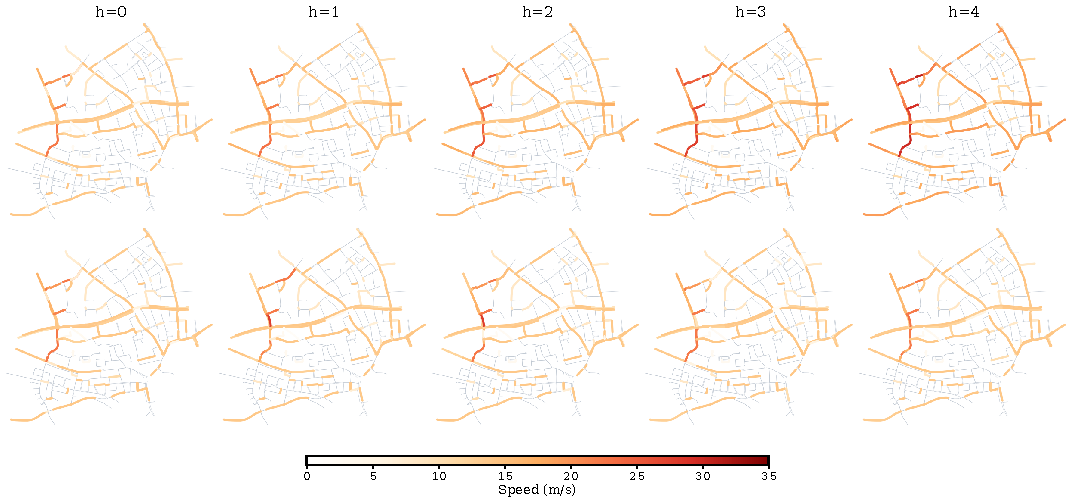
\includegraphics[width=0.75\linewidth]{figure/ingolstadt_construction.pdf}
    \caption{World-model rollout reconstruction on Ingolstadt. Top: speeds decoded from the predicted latent state. Bottom: simulator-observed segment speeds. Columns: prediction horizons \(h=0\) to \(h=4\).}
    \label{fig:ingolstadt-construction}
\end{figure}

\begin{figure}
    \centering
    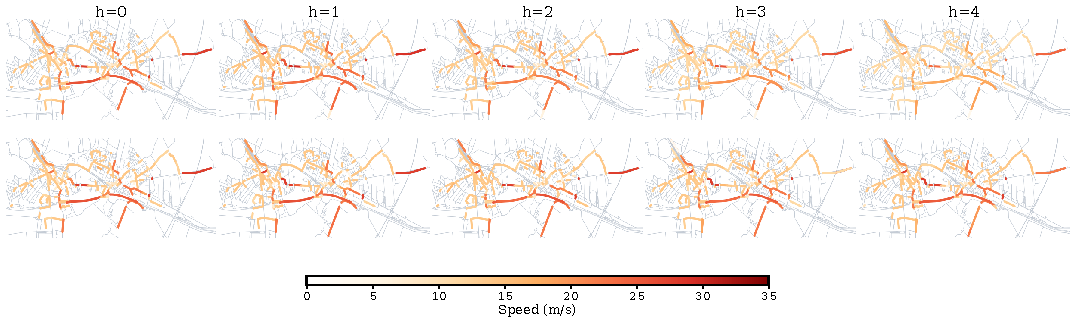
\includegraphics[width=0.75\linewidth]{figure/gretz_construction.pdf}
    \caption{World-model rollout reconstruction on Gretz-Armainvilliers, in the same layout as Figure~\ref{fig:ingolstadt-construction}.}
    \label{fig:gretz-construction}
\end{figure}

\begin{figure}
    \centering
    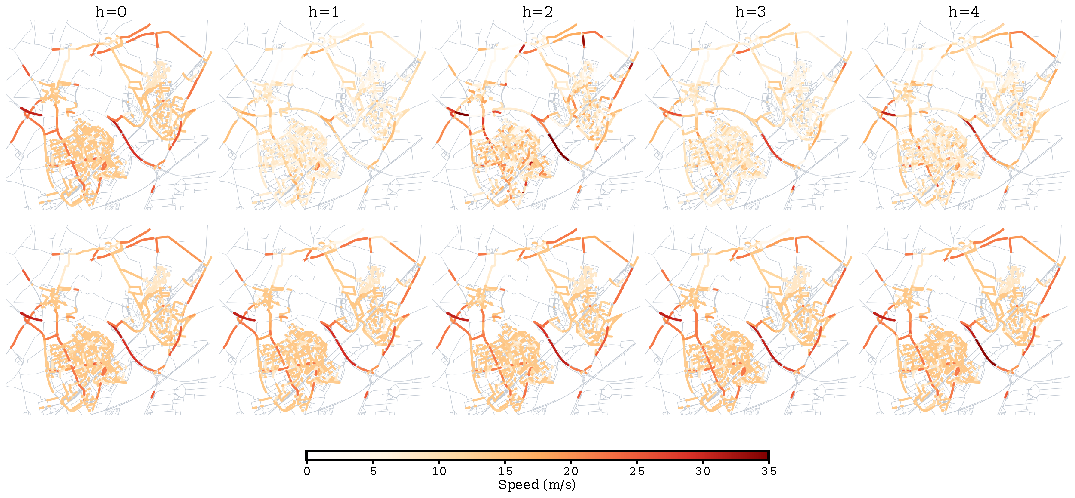
\includegraphics[width=0.75\linewidth]{figure/fontenay_construction.pdf}
    \caption{World-model rollout reconstruction on Fontenay-en-Parisis, in the same layout as Figure~\ref{fig:ingolstadt-construction}.}
    \label{fig:fontenay-construction}
\end{figure}


\end{document}
\endinput